\documentclass[pdftex,a4paper,halfparskip, article]{scrartcl}
% Andere Dokumentklassen: article, report, book, beamer, scrartcl, scrreprt, scrbook, beamer
% Prefix scr bedeuted aus dem KOMA-Script Paket, welches europäische Formatierungsstandards enthält
% Gebräuchliche Optionen sind: 11pt, 12pt, twoside, twocolumn, a4paper,...
\usepackage{ngerman} %Titel z.B. für Tabellen- und Inhaltsverzeichnis werden ins Deutsche übersetzt. Ausserdem Aktivierung der korrekten Silbentrennung
\usepackage{amsmath}

\usepackage{verbatim}
\usepackage[latin1, utf8]{inputenc} %Für das Erkennen von Umlauten

\usepackage[T1]{fontenc} %Font-Encodierung wird auf das T1-Format mit bis zu 256 (anstelle 128 im Default Fontencoder) umgeschaltet

\usepackage{hyperref}
\usepackage{graphicx}
\graphicspath{ {./images/} } 
\usepackage{color}

\title{Rapid Frontend Prototyping with Deep Learning} %Definition des Titels
\author{Simon Deussen}	%Definition des Autors
% \date{7.Nov.2010}

\begin{document}

\maketitle	

\begin{abstract}
Generierung von HTML/CSS Code für Websites aus Screenshots. Aufbauend auf dem Pix2Code Paper \cite{Beltramelli17}, ist diese Arbeit eine erweiterte Implementation mit mehr Elementen und damit komplexeren Websites. Ein Beitrag dieser Arbeit ist eine neue, verbesserte Netzwerk Architektur, als auch ein Tool, mit dem neue Trainingsdaten erzeugt werden können.
\end{abstract}


\tableofcontents	% Erstellung des Inhaltsverzeichnisses
%\listoffigures   % Abbildungsverzeichnis
%\listoftables    % Tabellenverzeichnis
\section{Einleitung} 

Worin besteht der Nutzen automatisierter Code erstellen? Besonders im Bereich der Frontend-Entwicklung, bei der ein Team aus Leuten mit unterschiedlichen Fertigkeiten benötigt wird, kann es bei der Entwicklung zu Bottlenecks kommen. In der klassischen Entwicklung sieht diese Zusammenarbeit folgendermaßen aus: \\
Ein Designer macht einen grafischen Entwurf, dieser wird vom Kunde abgenommen, dann geht er zu dem Entwickler, der nun zu aller erst Markup für den Content und anschließend das Design und die richtige Darstellung nach bauen muss. Für jede grafische Veränderung muss dieser Prozess wieder ausgeführt werden. Für die meisten Entwickler, ist die Markup und CSS-Erstellung der widrigste Part der ganzen Arbeit, da er recht zeit-aufwendig, repetitiv und langweilig ist.
Hier kommt es schließlich zu den Bottlenecks und Unzufriedenheit bei der Arbeit. Deswegen kann besonders ab der Schnittstelle zwischen Designern und Entwickler mit Automation viel gewonnen werden. Es gab bisher viele Ansätze diese Arbeit zu automatisieren, zum Beispiel durch Tools in dem man gleichzeitig Designen und den Markup exportieren kann. Leider sind diese Tools entweder nicht besonders gut darin, die Designs zu erstellen oder den Markup zu exportieren.

Eine Abhilfe soll diese Arbeit liefern: Sie ermöglicht, dass der Designer mit seinem bevorzugten Tools das Design entwickelt und der Entwickler mit einem Mausklick das fertige Markup bekommt. So kann sich der Entwickler vollends auf die Realisierung des Verhaltens und der Logik der Anwendung konzentrieren. 

\section{Ähnliche Arbeiten}

Diese Arbeit basiert auf dem Pix2Code Paper von Tony Beltramelli \cite{Beltramelli17}. Er war der erste der Code anhand von visuellen Input mit neuronalen Netzwerken generieren hat. 
Anderen Ansätze wie DeepCoder \cite{DeepCoder16} benötigen komplizierte DSL als Input und schränken so die Benutzbarkeit stark ein. Visuelle Versuche mit Android-GUIs von Nguyen \cite{Nguyen15} benötigt ebenfalls unpraktische von Experten erstellte Heuristiken. Pix2Code ist das erste Paper das einen allgemeinen Input hat, hier einfache Screenshots und diesen in drei verschiedene Targetsprachen übersetzten kann. Zum einen kann es HTMl/CSS Code erstellen, zum anderen aber auch Android- und iOS-Markup. Siehe Original Code auf Github \cite{Beltramelli17Github}


\section{Motivation}

Computer genierte Programme werden die Zukunft der Software Entwicklung sein und diesen Bereich auch grundsätzlich verändern. Schon jetzt im Bereich der Cloud mit Serverless Computing und Lambdas, geht es oftmals nur noch darum bestehende Software-Teile zu verbinden und zu konfigurieren. Diesen Trend, der eine Reduktion des Schreibens erreichen will und dazu stark in die Richtung des Konfigurierens geht, sehe ich in Zukunft noch viel umfassender und allgegenwärtiger. Es wird so weit gehen, dass man nicht nur wie hier in dieser Arbeit das Markup generiert sondern das aus einer Skizze sofort eine fertige Website gebaut wird, und man mit ein paar Klicks das nötige Verhalten einfach hinzufügen kann. 
Wobei dieser Trend nicht nur auf das Web bezogen ist. Ich denke das sich die Webtechnologien auch in der Desktop Umgebung durchsetzen.  Da Plattform unabhängig und sehr stark optimiert. Sehr einfach zu lernen, weit verbreitet. Zum Beispiel Electron \cite{electron} ermöglicht den einfachen Einsatz von Webtechnologien durch einen eingebettet Browser in der Desktopwelt.
Daher kommt die Motivation diese Arbeit zu verfassen: Automation ist unumgänglich, deswegen sollte man diese am besten selber bauen und damit endlosen Entwicklern das Leben leichter machen.

\section{Benutzte Technologien}

In dem folgenden Abschnitt werden die benutzten Technologien beschrieben. Diese Erklärungen sind recht generell und gehen zunächst nicht auf die genaue Verwendung der Technologien in dem Projekt ein, dies wird aber im Abschnitt ~\ref{sec:rfp} genauer beleuchtet.

\subsection{Neuronale Netzwerke}
Neuronale Netzwerke sind einfach zu benutzende Modelle, welche nicht-lineare Abhängigkeiten mit vielen latenten Variablen stochastisch abbilden können \cite{nnWebsite}. Im einfachen Sinne, sind sie gerichtete Graphen, deren Knoten oder Nodes aus ihren Inputs Werte errechnen und diese an die folgenden Nodes weitergeben. Hierbei werden zwischen 3 verschiedenen Arten von Nodes unterschieden:

\begin{description}
	\item[Input Nodes] Über diese Nodes bekommt das Netzwerke die Input Parameter.
	\item[Hidden Nodes] Nodes, welche das Netzwerke-interne Modell repräsentieren.
	\item[Output Nodes] Diese Nodes bilden die Repräsentation des Ergebnisses ab.
\end{description}

Nachdem die Node aus den Inputs einen Wert errechnet hat, geht dieser durch eine Aktivierungsfunktion. Diese Funktion stellt den Zusammenhang zwischen dem Input und dem Aktivitätslevel der Node her. Man unterscheidet zwischen folgenden Aktivitätsfunktionen

\begin{description}
	\item[Lineare Aktivitätsfunktion] Der einfachste Fall, linearer Zusammenhang zwischen Inputs und Output.
	\item[Lineare Aktivitätsfunktion mit Schwelle] Linearer Zusammenhang ab einem Schwellwert. Sehr nützlich um Rauschen herauszufiltern. Ein häufig genutzte Abhandlung davon:
	\begin{description}
		\item[ReLU] Hier werden nur der positive Werte weitergeleitet: \(f_x = x^+ = max(0,x) \)
	\end{description}
	\item[Binäre Schwellenfunktion] Nur zwei Zustände möglich: 0 oder 1 (oder auch -1 oder 1)
	\item[Sigmoide Aktivitätsfunktion] Benutzung entweder einer logistischen oder Tangens-Hyperbolicus Funktion. Diese Funktionen gehen bei sehr großen Werten gegen 1 und bei sehr negativen Werten gegen 0 (logistische Funktion) oder -1 (Tangens-Hyperbolicus Funktion). Diese Funktion bietet den Vorteil das sie das Aktivitätlevel begrenzt.
\end{description} 

Jede der Nodes hat eine bestimmte Anzahl an Verbindungen, diese hängt von der Art der Nodes und deren Zweck ab. Wichtig ist jedoch, das jede Node mit mehreren anderen Nodes verbunden ist, dies soll heißen, den Output mehrerer Nodes als Input zu bekommen und den eigenen Output als Input für die folgenden Nodes weiterzuleiten. Die Stärke der Abhängigkeit zwischen zwei Nodes wird als Gewicht ausgedrückt. Jede Verbindung in einem Neuronalen Netzwerk hat ein Gewicht, welches mit dem Output der vorangegangen Node multipliziert wird bevor es als Input weiter verwendet wird.

Das Netzwerk-interne Modell wird in diesen Gewichten abgespeichert. Es repräsentiert also das Wissen, dass durch das Training entstanden ist.

Das Training eines Netzwerkes ist das schrittweise Anpassen der Gewichte bis es ein gutes Modell des Problems gelernt hat. Die Stärke von neuronalen Netzen liegt darin, aus großen Mengen von Daten Gesetzmäßigkeiten oder Patterns zu erkennen. Ein einfaches Beispiel ist die Objekterkennung. Wenn ein Netzwerk Alltagsgegenstände erkennen soll, lernt es die Pixelgruppen, welche ein Tisch von einem Bett unterscheiden. Damit dies funktioniert braucht man eine große Menge an Daten. Zunächst wird das Training in zwei verschieden Arten unterteilt: 

\begin{description}
	\item[Supervised learning] Innerhalb des Trainingsdatensets, hat jeder Datensatz einen vorgegeben Output Label. Zum Beispiel ein Bild von einem Auto ist auch so gekennzeichnet. Nun werden so lange die Gewichte des Netzwerkes optimiert, bis ein jeweiliger Input auch den richtigen Output erzeugt.
	\item[Unupervised learning] Hier hat das Trainingsdatenset keine Label. Die Gewichtsveränderungen erfolgen im Bezug zur der Ähnlichkeit von Inputs. Das soll heißen, wenn es viele verschiedene Bilder bekommt, werden Bilder mit ähnlichen Inhalten eine hohe Nähe aufweisen, ein Bild von einem PKW wird näher an dem Bild von einem LKW sein als an dem Bild von einem Apfel.
\end{description}

\subsection{Convolutional Neural Network - CNN}

CNN sind Tiefe neuronale Netzwerke mit einer bestimmten Architektur und spezialisiert auf die Verarbeitung von Bildern. Da man die Anwendungsdomäne eingeschränkt hat, kann man bestimmte Annahmen treffen, welche die Anzahl der Verbindungen und damit Rechenoperationen verringert und somit das Netz effektiver macht. Um aus Bildern, Informationen zu gewinnen, müssen die Ebenen des Netzwerkes nicht vollständig verbunden sein. Stattdessen werden Filter (Convolutions) und Sub-Sampling genutzt \cite{colahsBlogCnn}. Filter sind kleine Matrizen, die bestimmte Features entdecken, zum Beispiel Kanten mit bestimmter Ausrichtung. Durch das Erlernen der Filter im Training kann das Netzwerk aus den Pixelwerten, schrittweise abstraktere Features errechnen. Diese gehen von einfachen Kanten, zu komplexeren Umrissen, und schließlich zu vollständigen Teil-Objekten . Zum Beispiel werden aus vielen Kanten ein Kreis, aus mehreren einfachen Objekten ein detaillierter Umriss und schließlich entsteht aus den einfachen Features eine Repräsentation eines Kopfes.
Diese geschichtete Architektur ist von dem Auge und der biologischen Signalverarbeitung inspiriert \cite{Hubel68}. Einzelne Neuronen des celebralen Kortex reagieren auf Reize nur in einem beschränkten Bereich. Da diese Bereiche leicht überlappen können so diese Neuronen den gesamten Sichtbereich erkennen. 

\begin{figure}[h]
\centering
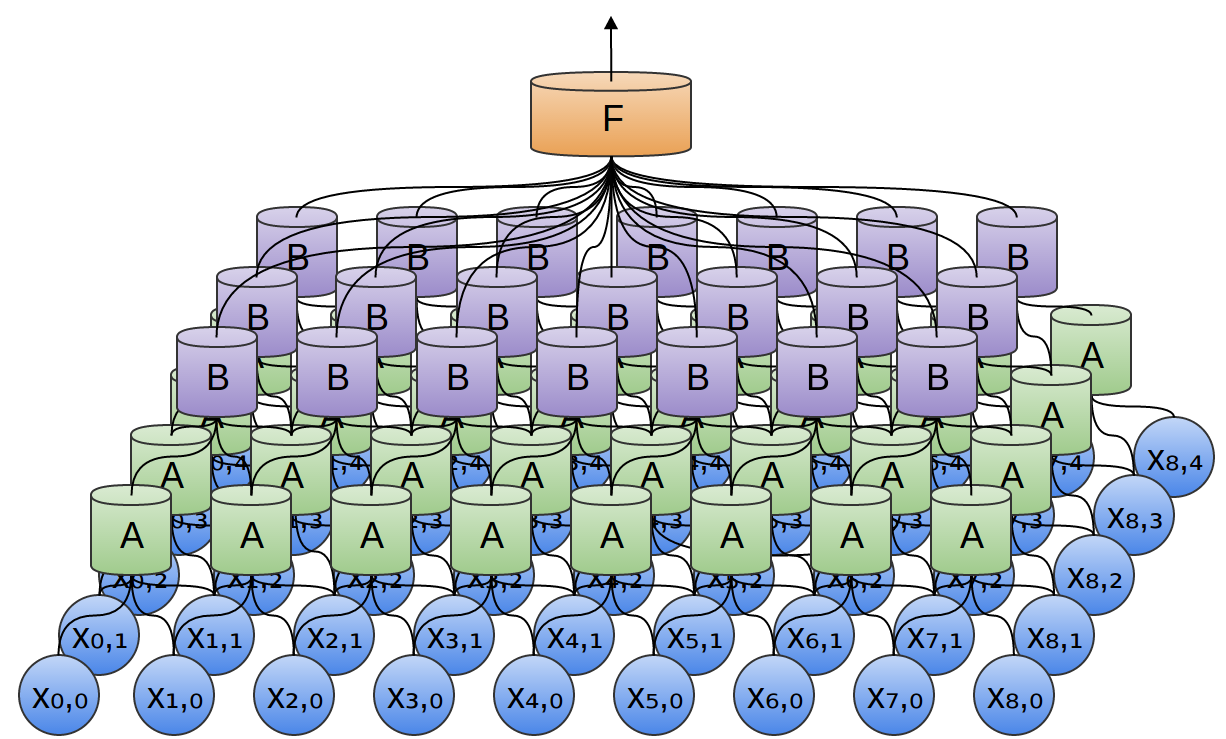
\includegraphics[width=0.5\textwidth]{colah_cnn}
\caption{CNN von \url{http://colah.github.io/}}
\label{fig:colah-cnn}
\end{figure}


In Neuronalen Netzen sind Fully-Connected-Layer die Ebenen mit den meisten Verbindungen. Bei Betrachtung der Abbildung~\ref{fig:colah-cnn}, würde eine Fully-Connected-Layer insgesamt $ n = 9^2 * 5^2 = 2025$ Verbindungen zwischen $x_{i, j}$ und $A$ benötigen. Stattdessen benötigen die Convolutional-Ebene mit einem Kernel von $2*2$ nur $n = 8 * 5 *4 = 128$ Verbindungen. Abgesehen von den Einsparung der Verbindungen, hat ein CNN viele verschiedene Kernel, welche sich pro jeweils die gelernten Gewichte teilen \cite{colahsBlogCnn}. Für jeden Kernel $A$ in der Abbildung werden die gleichen 4 Gewichte gebraucht. Diese Gewichte werden während dem Training gelernt und bilden dann ein bestimmtes Feature der Input-Daten ab, wie oben beschrieben.

\begin{figure}
\centering
\begin{minipage}{.5\textwidth}
  \centering
  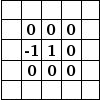
\includegraphics[width=.3\linewidth]{gimp_doku_edges_kernel}
\end{minipage}%
\begin{minipage}{.5\textwidth}
  \centering
  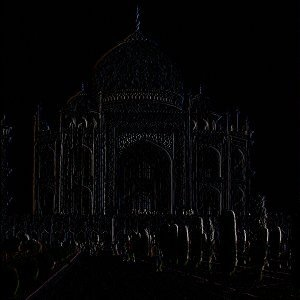
\includegraphics[width=.8\linewidth]{gimp_doku_edges}
  \end{minipage}
\captionof{figure}{Beispiel Kernel aus der Gimp-Dokumentation \cite{gimpdoku}}
  \label{fig:kernel}
\end{figure}

Die Operationen die Kernel auf einem Input ausführen, ist in Abbildung~\ref{fig:kernel} visualisiert. Hier wird durch eine einfache Convolution eine Repräsentation des Inputs gebildet, in der nur vertikale Kanten enthalten sind. Wenn nun ein Kernel mit einer derartigen Operation in Netzwerk aktiviert wird, teilt dieser dem Rest des Netzwerkes mit, dass hier eine vertikale Kante in Input ist.

Durch das Kopieren der Kernel und der geringeren Verbindungsanzahl sind nun sehr große und sehr tiefe Modelle möglich. In 2012, haben Krizhevsky et al. die Welt der Bildklassifizierung mit ihrem Paper und den darin vorgestellten Modell revolutioniert \cite{ImageNetOriginal}. Ihr tiefes, convolutional Neural Network konnte insgesamt 1000 Klassen unterscheiden mit einer Genauigkeit von 63\%. Deren Ergebnisse waren der Anfang einer neuen Art von Bildklassifizierung und es folgten viele weitere Paper die auf deren Erfolg aufbauend, CNNs tief in der Computer Vision verankerten \cite{colahsBlogCnn}.

\subsection{Recurrent Neural Network - RNN}

RNNs sind eine Erweiterung der klassischen Feedforward Netze, die imstande sind, Input-Sequenzen mit verschiedener Länge zu verarbeiten \cite{paperGRUComparison}. Die RNN schaffen dies, in dem sie einen inneren Zustand haben, dessen Aktivierungen von vorherigen Inputs abhängig sind. 
RNNs haben Verbindungen zu Neuronen der selben oder vorhergehenden Schichten und können dadurch Inputs durch das gesamte Netz durchgeben. 

\begin{figure}[h]
\centering
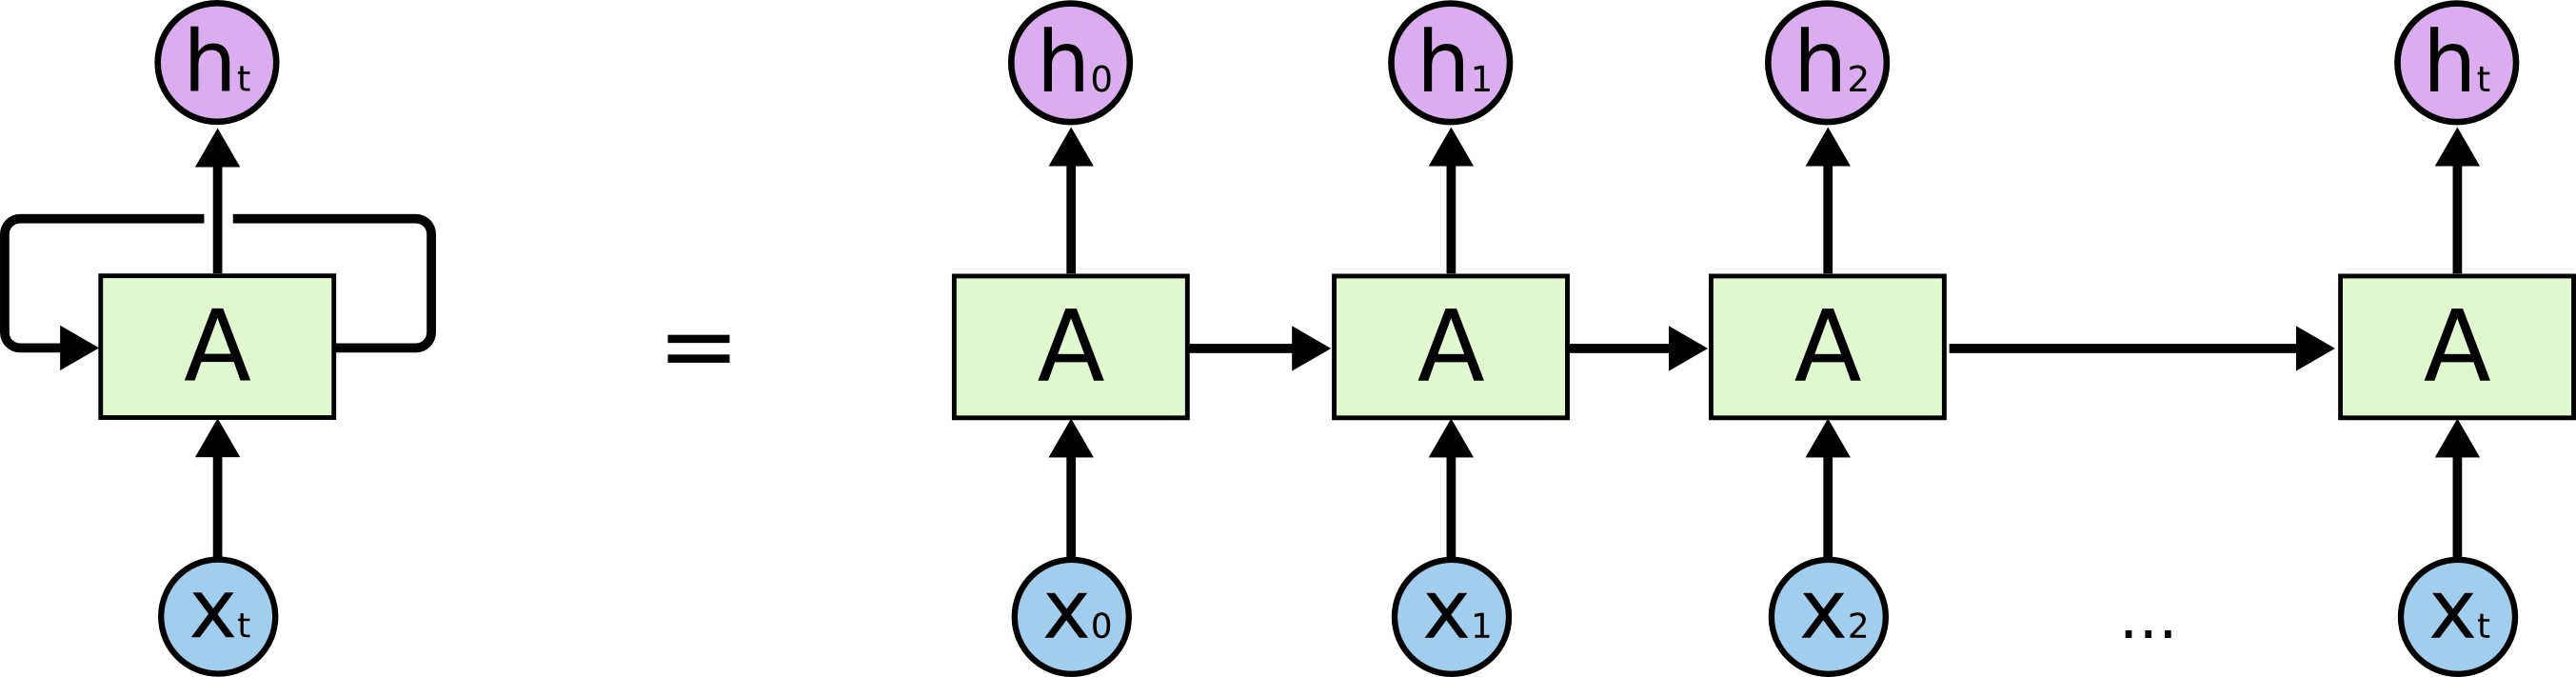
\includegraphics[width=0.5\textwidth]{colah_rnn}
\caption{RNN von \url{http://colah.github.io/}}
\label{fig:rnn}
\end{figure}

Wie auf der Abbildung~\ref{fig:rnn} zu sehen ist, ähnelt der Verbund der rekurrenten Einheiten einer Liste. Damit ist diese Art Neuraler Netzwerke besonders gut geeignet sequentielle Daten abzuarbeiten \cite{colahsBlogLSTM}. Listen, Sprachsynthese und maschinelle Übersetzungen sind Bereiche wofür RNNs gut geignet sind. Klassische RNNs, gelangen jedoch an einen Punkt, ab dem sie Sequenzen von zu großer Länge nicht mehr ausreichend gut modellieren können, da aber einer gewissen Länge, beim Training die Gradienten zu numerischer Instabilität neigen \cite{DBLP:journals/corr/Graves13}. Das heißt, die Gradienten gehen gegen null oder in seltenen Fällen gegen $\infty$ \cite{paperGRUComparison}, wodurch das Training scheitert. Damit scheidet das reine Verketten von RNN-Units aus, um lange Abhängigkeiten zu modellieren. 

\subsubsection{Long short-term Memory - LSTM}

Ein LSTM ist eine bestimmte Form der RNNs. Ein LSTM ist so gebaut, dass die einzelnen Units selber entscheiden können, welche Daten beibehalten oder vergessen werden - es hat einen eigenen Speicher, dessen Benutzung und Verwaltung von dem LSTM während dem Training gelernt wird. Durch diese dynamische Speicherverwaltung, kann es auf der einen Seite, bestimmte Informationen länger speichern, auf der anderen, kurzfristig benötigte Daten verarbeiten und dann wieder vergessen. Ein einfaches Beispiel ist ein Text-verarbeitendes LSTM. Dieses LSTM hat die Aufgabe aus Texten Informationen über Autos zu extrahieren. Sobald es in dem Text um ein anderes Auto der gleichen Marke geht, kann das LSTM, die Bezeichung des Autos, die Farbe und Zylinderanzahl des Motors vergessen, da die bei dem nächsten Auto verschieden sind. Die Marke hingegen bleibt direkt gespeichert und abruf bereit. 

Während des Trainings eines LSTMs, erlernt dieses auch das Speichern und Löschen. Dadurch kann es sehr viel effizienter als reine RNNs Daten mit temporaler Dimension oder langen Abhängigkeiten auswerten. Fast jeder Erfolg, der mit RNNs erzielt wurde, ist auf LSTMs zurückzuführen \cite{colahsBlogLSTM}. 

Eingeführt wurde das LSTM von Hochreiter und Schmidhuber im Jahr 1997 \cite{LSTM_orig}. Seit dem wurden viele Variationen davon getestet, verworfen und verbessert. In dieser Arbeit wird mit dem Begriff LSTM diese Original Spezifikation gemeint.

\begin{figure}[h]
\centering
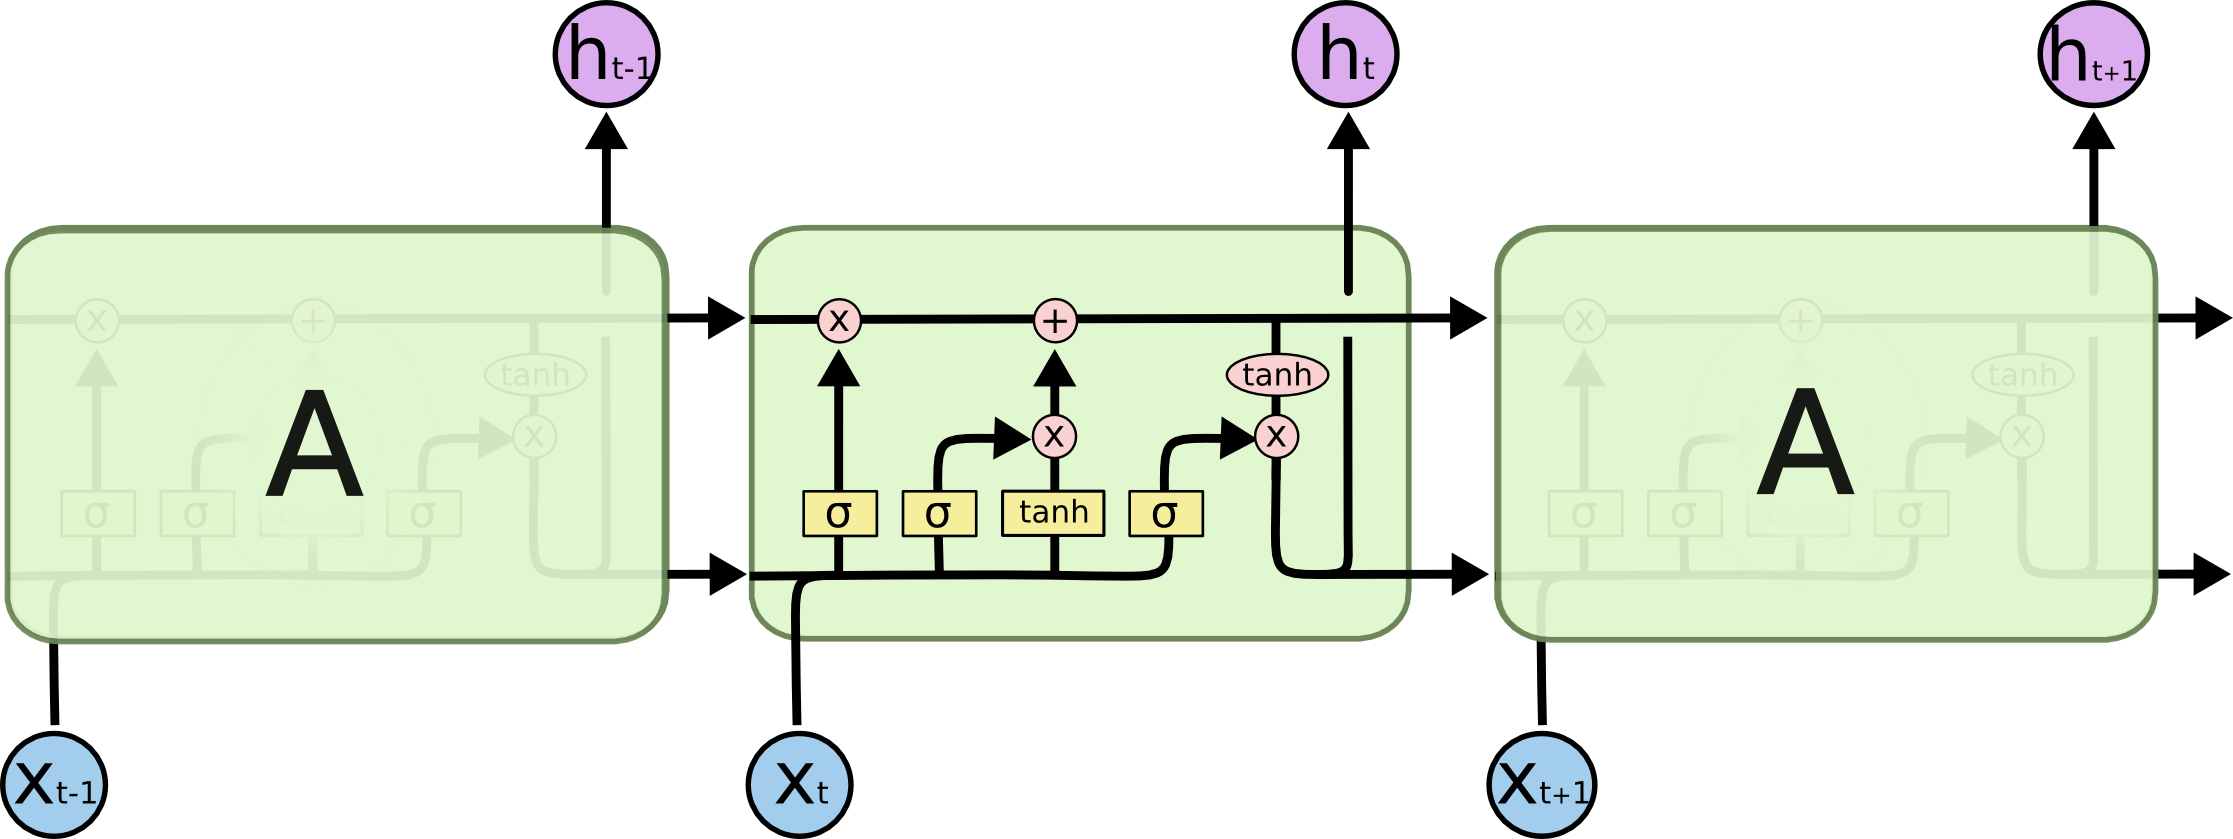
\includegraphics[width=0.5\textwidth]{colah_lstm}
\caption{LSTM von \url{http://colah.github.io/}}
\label{fig:gru}

\end{figure}

Eine LSTM-Unit teilt sich mit allen anderen LSTM-Units des Netzwerkes einen Cell-State, in der Abbildung die obere, horzontale Linie. Jede Unit kann diesen auf zwei Arten verändern, mit einem \texttt{forget}-Gate werden Informationen vergessen, mit einem \texttt{add}-Gate Informationen hinzugefügt. Schließlich berechnet jede Unit einen eigenen Hidden-State anhand des Inputs, des geteilten Cell-States und dem Hidden-State vorangegangener Units.


\subsubsection{Gated Recurrent Unit - GRU}

Die GRU, ist eine Abwandlung des klassischen LSTM. Die Architektur wurde 2014 von Kyunghyun Cho et al. eingeführt \cite{DBLP:journals/corr/ChoMGBSB14} um eine RNN Einheit zu erhalten, welche es schafft selbstständig Feautures aus verschiedenen, weit auseinander liegenden, Zeitpunkten zu extrahieren \cite{paperGRUComparison}. Was diese Variante ausmacht, ist eine Zussammenführung des \texttt{forget}- und \texttt{add}-Gates, sowie das Weglassen des Cell-States. Dadurch hat es weniger Parameter als die klassische Variante.
\begin{figure}[h]
\centering
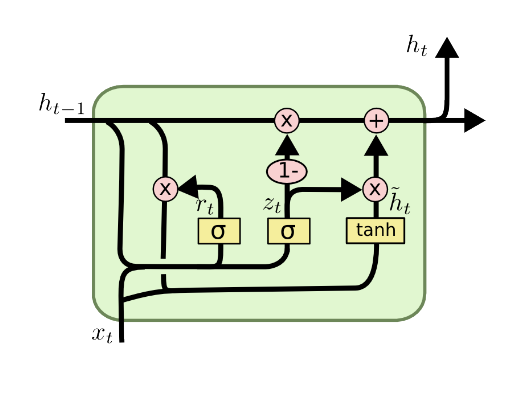
\includegraphics[width=0.3\textwidth]{colah_gru_small}
\caption{GRU von \url{http://colah.github.io/}}
\end{figure}
Trotz der geringeren Anzahl an Parameter, ist die Performance ähnlich der klassischen Variante\cite{lstmSearchSpace}, trainiert aber schneller, da weniger optimiert werden muss.  Im LSTM erfolgt eine Kontrolle darüber, wie viel des Cell-States mit in einer Berechnung einfließt. Im GRU auf der andern Seite, wird immer die volle Historie mit in die Berechnung aufgenommen \cite{paperGRUComparison}. 


\subsection{Training}

Als Training wird der Prozess bezeichnet, während dem ein Neurales Netzwerk Wissen aus vorliegenden Daten extrahiert. Genau dieser Vorgang sorgt für den großen Erfolg von Neuralen Netzen. Anders als bei herkömmlichen statistischen Methoden können NNs aus riesigen Datenmengen Patterns und Sachverhältnisse lernen. Damit dies funktioniert, muss eine Kostenfunktion gebildet werden können, anhand bestimmt wird, wie weit das genutzte Modell von der optimalen Lösung entfernt ist. Anhand diesem Abstand, können die Parameter des gewählten Modells angepasst werden, um dem Optimum näher zu kommen.

\subsubsection{Overfitting}
	
Overfitting tritt ein, wenn das Modell zu Komplex für den gewählten Task ist, und deswegen die Trainingsdaten auswendig lernt. Somit wird es sehr gute Ergebnisse auf dem Trainingsset zeigen, sobald es aber Daten bekommt, die es nicht kennt, wird die Performance abstürzen, da es nicht Verallgemeinern kann. Eine Art Overfitting zu lösen, ist es das Netzwerk zu verkleinern oder spezielle Ebenen wie Dropouts einzubauen, die dem entgegen wirken.

\subsubsection{Underfitting}

Dies ist das Gegenteil von Overfitting; das Netzwerk schafft es nicht ein Modell zu finden um das Problem zu approximieren, da es zu einfach aufgebaut ist. Eine gängige Lösung ist es, das Netzwerk zu vergrößern damit es das komplexe Problem besser lösen kann.


\subsubsection{Stochastig Gradient Descent - SGD}

SGD ist eine iterative Methode um ableitbare Funktionen und Modelle zu optimieren. Um ein Modell zu optimieren, wird eine Verlustfunktion benötigt. Diese zeigt den Schaden an, der entsteht wenn das Modell mit falschen Parametern Entscheidungen trifft. Um die richtigen Parameter während des Trainings zu finden, muss diese Verlustfunktion minimiert werden.
Bei SGD werden durch zufällige Samples des Trainingssets, Näherungen an den Gradienten gebildet, die dann wiederum genutzt werden um die Parameter zu optimieren. Nach mehreren Durchläufen durch das Trainingsset wird ein Set an Parameters gefunden, die ein Minimum der Verlustfunktion bilden \cite{walkSGD}. 


\begin{description}
	\item[RMSprob] Eine Variante des SGD, die sich besonders gut eignet um RNNs zu optimieren \cite{kerasDocRMSprob}. Diese wird in der Arbeit genutzt.
\end{description}

\subsubsection{Dropout}

Dropout ist eine Technik, die genutzt wird um Overfitting zu vermeiden. Während des Trainings werden zufällig Nodes sowie ihre Eingangs- und Ausgangsverbindungen aus dem Netzwerk entfernt \cite{JMLR:v15:srivastava14a}.

\subsubsection{Transferlernen}

Transferlernen ist ein Process, bei dem ein fertiges Netzwerk, welches auf ein bestimmtes Problem trainiert ist, für ein andere Problemlösung genutzt wird. Anstatt das Netzwerk mit zufälligen Gewichten zu verwenden, werden die bereits erlernten Gewichte weiter trainiert bis diese gelernt haben, das neue Problem zu lösen. Gerade im Bereich der Bildklassifizierung ist diese Technik sehr sinnvoll, da allgemeine Features wie verschieden ausgerichtete Kanten oder einfache geometrische Objekte universell sind und so nicht erst gelernt werden müssen. So hat das Netzwerk eine gewisse Wissensbasis die für die neue Problemdomäne als Grundbaustein dient.

\subsection{Sampling}
Während dem Sampling, wird ein fertig trainiertes Neurales Netzwerk genutzt um, aus Daten Schlussfolgerungen abzuleiten. In dem Fall dieser Arbeit, wird probiert aus einem Screenshot, eine deutungsvolle DSL-Sequenz zu erstellen.

\subsection{Keras}
Um die in dieser Arbeit genutzten Tiefen neuronalen Netzwerke zu definieren wir das Framework Keras \cite{chollet2015keras} genutzt. Keras ist eine Library, die es sehr einfach macht Neuronale Netzwerke zu erstellen und verwalten. Es selber verwaltet nur die Definition von Modellen, die eigentlichen Berechnungen werden im Backend getätigt, von Theano, Tensorflow oder CNTK. So ermöglich es schnelles experimentieren mit wenig Overhead und keinen Boilerplate-Code. 

\subsection{Domain-specific language - DSL}

Eine Programmiersprache, die auf ein einzelne Problem-Domäne spezialisiert ist, wird DSL genannt. Im Gegensatz zur DSL steht die General Purpose Language, welche ein Programmiersprache ist, die sehr breit, für viele verschiedene Anwendungen, benutzt werden kann. Die Trennung zwischen DSL und GPL ist nicht immer klar, es kann zum Beispiel Teile einer Sprache geben die hoch spezialisiert für eine bestimmte Aufgabe sind, aber andere Teile von ihr können allgemeinere Aufgaben lösen. Auch historisch bedingt kann sich die Einordnung einer Sprache ändern. JavaScript wurde ursprünglich für ganz einfache Steuerung von Websites eingeführt, kann aber inzwischen für alles mögliche eingesetzt werden - vom Trainieren von CNNs im Browser, zu klassischen Backend-Jobs. 
In dieser Arbeit, wird eine hoch spezialisierte, eigens erstellte Sprache aus Token, die eine Kombination aus HTML und CSS sind, benutzt.

\subsubsection{Hypertext Markup Language - HTML}
HTML ist die Standardprogrammiersprache um Websites zu erstellen. Mit einzelnen HTML Elementen beschreibt es den semantischen Zusammenhang des Contents von Websites.

\subsubsection{Cascading Style Sheets - CSS}
CSS beschreibt die Präsentation, also das Aussehen, des Content einer Markup-Language (zum Beispiel HTML). Klassische Inhalte, sind Farben, Positionen und Effekte von User Interface Elementen.
 

\section{Rapid Frontend Prototyping - Überblick}\label{sec:rfp}

RFP ist ein Tool, welches aus einfachen Website-Screenshots HTML/CSS Markup erzeugen kann. Dafür lernt ein System aus Neuralen Netzwerken eine einfache Domain Specific Language (DSL). Jeder Token in dieser Sprache hat zugehörigen HTML/CSS Code, wodurch eine Token-Sequenz einfach in diese Sprache kompiliert werden kann.

Um den Code für die Website Screenshots zu generieren, wird ein Modell bestehend aus 2 rekurrenten Netzwerken und einem Convolutional Neural Network erstellt. Das hier genutzte Modell ist eine Abwandlung des im Original Paper verwendeten Modells. Da die neue DSL komplexer als die im Original Paper\cite{Beltramelli17} ist, musste sowohl das CNN als auch die RNNs verändert werden. 

Von einem Computer abgespeicherte Bilder sind ein denkbar schlechtes Format um aus den Rohdaten auf deren Inhalte zuschließen. Die Pixel, die einem Bild zugrunde liegen, sind lediglich Helligkeitsinformationen, die zwar einfach genutzt werden können, um für Menschen Bilder darzustellen, aber in roher Form eben sehr wenig Informationen enthalten, was in einem Bild dargestellt wird. Um aus diesem Zahlenwerten Schlussfolgerungen zu schließen, müssen diese in mehreren Schritten abstrahiert werden, um bedeutungsvolle Features zu extrahieren. Hierfür wird ein CNN genutzt. Dieses verarbeitet das gegebene Input-Bild und erstellt eine niedrig-dimensionale Repräsentation. Die Architektur des CNN ist angelehnt an das VGGNet von Simonyan and Zisserman \cite{DBLP:journals/corr/SimonyanZ14a}.

Das erste RNN, wird dafür benötigt, um die DSL zu lernen, insbesondere die validen Reihenfolgen und die Grammatik. Das zweite RNN, bekommt als Input, den Output des CNN, also eine Repräsentation des Bildes sowie den Output des ersten RNNs. Daraus kann es wiederum eine valide Tokenabfolge generieren die den Screenshot beschreibt. Zu sehen ist dieses Zusammenspiel in der Abbildung~\ref{fig:pix2code_paper_architecture}.

\begin{figure}[h]
\centering
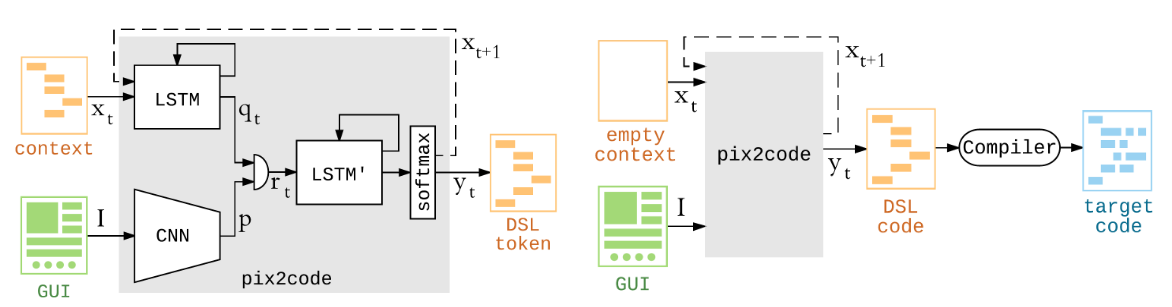
\includegraphics[width=0.95\textwidth]{pix2code_paper_architecture}
\caption{Architektur des Netzwerkes, Grafik aus dem Original Paper \cite{Beltramelli17}}
\label{fig:pix2code_paper_architecture}
\end{figure}

Die rechte Seite der Abbildung~\ref{fig:pix2code_paper_architecture} stellt den Zustand während dem Training dar. Ein Screenshot, zusammen mit der dazugehörigen Token Sequenz wird als Input in das Netzwerk angelegt. Die Details hierzu sind in Section~\ref{sub:training}. Nachdem das Training fertig ist, wird ein Input, an das Modell angelegt, der nur einen \texttt{Start}-Token enthält. Dieser leere Kontext wird nun Token, für Token, von dem Modell befüllt, bis ein \texttt{End}-Token erzeugt wird. Auf der rechten Seite der Abbildung~\ref{fig:pix2code_paper_architecture} sieht man die Generierung. Dem anfangs leeren Kontexts wird jeder weitere generierte Token hinzugefügt. Das Netzwerk bekommt so den eigenen Output wieder als Input. Dies ist eine gängige Methode um ein Netzwerk zu nutzen, um Sequenzen von unterschiedlicher Länge zu generieren \cite{DBLP:journals/corr/Graves13}.

\subsection{Vision Modell}
 
CNN ermöglichen eine aussagekräftige Repräsentation eines Inputs, hier eines Screenshots, zu erlernen. In dieser Arbeit findet das CNN des Modells durch unüberwachtes Lernen eine derartige Repräsentation der Screenshots. Die Screenshots werden wir um Original Paper auf 256 mal 256 Pixel herunter skaliert, ohne Bewahrung der Seitenverhältnisse. Ähnlich des VGGNets \cite{DBLP:journals/corr/SimonyanZ14a} nutzt das CNN Convolutions mit einem 3 mal 3 Pixel großen Kernel, welche über ein ReLU aktiviert werden. Die 3x3 Convolution Ebenen werden jeweils zweimal hintereinander genutzt. Anschließend wird eine Pooling Ebene genutzt und ein Dropout ausgeführt. Wie im Code zu sehen ist, wird die Anzahl der Features pro \texttt{Conv2D/Conv2D/MaxPooling2D/Dropout}-Modul jeweils verdoppelt.

\begin{verbatim}
image_model = Sequential()
image_model.add(Conv2D(32, (3, 3), padding='valid', activation='relu', 
input_shape=input_shape))
image_model.add(Conv2D(32, (3, 3), padding='valid', activation='relu')) 
image_model.add(MaxPooling2D(pool_size=(2, 2)))
image_model.add(Dropout(0.25))

image_model.add(Conv2D(64, (3, 3), padding='valid', activation='relu'))
image_model.add(Conv2D(64, (3, 3), padding='valid', activation='relu'))
image_model.add(MaxPooling2D(pool_size=(2, 2)))
image_model.add(Dropout(0.25))

image_model.add(Conv2D(128, (3, 3), padding='valid', activation='relu'))
image_model.add(Conv2D(128, (3, 3), padding='valid', activation='relu'))
image_model.add(MaxPooling2D(pool_size=(2, 2)))
image_model.add(Dropout(0.25))

image_model.add(Flatten())
image_model.add(Dense(1024, activation='relu'))
image_model.add(Dropout(0.3))
image_model.add(Dense(1024, activation='relu'))
image_model.add(Dropout(0.3))

image_model.add(RepeatVector(CONTEXT_LENGTH))
\end{verbatim}

Danach werden 2 Fully-Connected Ebenen (\texttt{Dense} im Code) genutzt. Anschließend wird der Output über den \texttt{RepeatVector} an das Decoder-RNN weitergegeben.

\subsection{Sprach Modell}

In diesem Teil des Netzwerkes wird eine Netzwerk-interne Repräsentation der DSL erlernt. Damit das Netzwerk die DSL verstehen kann, wird diese per One-Hot-Encoding übergeben. Weder die Repräsentation als String, noch die als One-Hot-Encoding gibt den einzelnen Token eine Bedeutung. Genau dafür wird das Sprach-Modell benötigt, denn die Netzwerk-interne Repräsentation, erschafft eine detaillierte Sprache, welche ähnlich, den Features aus höheren CNN Ebenen mehr Informationen enthält. 

Realisiert wird das Sprach-Modell durch zwei Ebenen aus rekurrenten Units. Im Original Paper wurden hier LSTM Units benutzt, in der Implementation dieser Arbeit jedoch GRU Units. Beides rekurrenten Units unterscheiden sich hauptsächlich in der internen Verwaltung vorheriger Zustände und der Modellierung von längeren Beziehungen in den Input-Daten \cite{colahsBlogLSTM}. 

Das Sprach Modell, gibt nach der Enkodierung des Sprach-Inputs, diesen an das Decoder-Modell weiter. Während des Trainings, erhält das Sprach-Modell einen Input Vektor, gefüllt mit dem \texttt{start}-Token und dem ersten Token der zu dem Screenshot passenden Token-Sequenz. Dieser Vektor arbeitet mit einem Sliding-Windows alle Tokens der Token-Sequenz ab, bis der gesamte Content an das Netzwerk übergeben wurde. Im Falle der Generierung von Code, wird dem Sprach-Modell in der ersten Iteration ein leerer Vektor, nur mit dem \texttt{start}-Token gefüllt übergeben. Dieser Vektor wird nun mit iterativ mit den Outputs des Netzwerkes befüllt, wie das Netzwerk den \texttt{end}-Token generiert.

Diese Ebenen geben als Output die gesamte Verarbeitete Sequenz zurück. Dadurch hat dieser Output die Maße $\texttt{CONTEXT\_LENGTH} * \texttt{ANZAHL\_RNN\_UNITS}$. J


\subsection{Decoder Modell}



Der Decoder-Teil des generiert aus dem zusammengefügten Outputs des Vision- und des Sprach-Modells die Token-Sequenz. Übergeben werden die Daten folgendermaßen: \texttt{decoder = concatenate([encoded\_image, encoded\_text])
}. Durch die \texttt{concatemate}-Funktion, wird jeder einzelne kodierte Sprach-Output mit einer Repräsentation des Screenshots verknüpft.  Nachdem der Input Screenshot sowie die dazugehörigen Tokens verarbeitet wurden, muss das Netzwerk nun den Zusammenhang zwischen diesen Daten erlernen. 

Auch dieser Teil des Netzwerkes besteht aus rekurrenten Units. Zum Vergleich, dieser hier hat viermal so viele Einheiten wie das Sprach Modell. Auch hier wurden bessere Ergebnisse bei der Benutzung von GRUs anstellte von LSTMs erzielt.

Nachdem die Input-Daten von den beiden anderen Teilen des Netzes in eine Repräsentation derselben umgewandelt wurden, müssen diese Token für Token wieder in ein One-Hot-Encoding übersetzt werden. Das Decoder-Modell bekommt als Input gleichzeitig den Screenshot sowie im Falle des Trainings einen kodierten Ausschnitt aus der echten Sequenz oder im Falle des Generierens die einen kodierten Ausschnitt der bisher vorhergesagten Tokens. Aus diesen beiden Daten erstellt es nun solange den nächsten bis das Modell die Annahme findet, dass der Inhalt abgearbeitet wurde. In diesem Fall wird der \texttt{end}-Token generiert und das Generieren wird eingestellt.


\subsection{Mathematische Beschreibung}

Mathematisch gesehen lässt sich die Generierung von Tokens durch das Netzwerk folgendermaßen beschreiben:

\begin{equation}
\begin{aligned}
encImg  &= CNN(inputImg) \\
encTkn &= RNN(token_t) \\
predToken &= softmax(RNN'(encImg, encTkn)) \\
token_{t+1} &= token_{t+1} + predToken
\end{aligned}
\end{equation}


\begin{description}
	\item[$inputImg$] Screenshot der Website, $256 * 256$ Pixel.
	\item[$encImg$] Encoding des CNNs vom Input Bild, durch die abschließende \texttt{RepeatVector}-Ebene, sind die Output-Maße $\texttt{CONTEXT\_LENGTH} * 1024$. 
	\item[$token_t$] Entweder der zuletzt vorkommende Token, oder beim Start der Prediction, ein \texttt{Start}-Token. Output der Maße $\texttt{CONTEXT\_LENGTH} * \texttt{ANZAHL\_TOKEN}$, Häufig auftrendender Fall: $48 * 23$ 
	\item[$encTkn$] Die Modell-interne Repräsentation der Tokens
	\item[$predToken$] Ausgabe des Netzwerkes. Wird für den nächsten Schritt an den Input hinzugefügt.
	\\
	\item[$CNN$] Der Vision-Teil des Modells
	\item[$RNN$] Das Sprach-Modell
	\item[$RNN'$] Der Encoder-Teil des Modells
\end{description}

Durch die Verkettung der jeweiligen Netzwerke ist die Gesamtarchitektur nach wie vor ableitbar und damit von Anfang bis Ende optimierbar. 

\section{Daten Synthese}

Da im Zuge dieser Arbeit eine Erweiterung der DSL des Original Papers implementiert wurde, ist es erforderlich, neue Trainingsdaten zu synthetisieren. Ein Beispiel eines der neu synthetisierten Daten ist in der Abbildung~\ref{fig:beispiel_daten} zu sehen. Im Zuge der Arbeit wurden insgesamt 4 verschiedene Datensets synthetisiert, mit jeweils ca. 3000 bis 4000 Bildern. 

Das DataCreationTool ist ein Programm, welches nach vorgegebenen Regeln einen Token-Baum erzeugt und diesen anschließend abspeichert. Dieser Token-Baum hat immer einen body-Token als Wurzel und der gesamten Inhalt liegt als dessen Kinder vor. Dafür wurde eine Helferklasse geschrieben, die ein Element in dem Token Baum abbildet. Diese kann zum einen Parameter wie den Token-Name, Inhalt und Kinder speichern, zum anderen enthält sie Funktionen zum Konvertieren des Baumes zu einer String-Repräsentation sowie zum Rendering nach HTML/CSS. 

\begin{figure}[h]
\centering
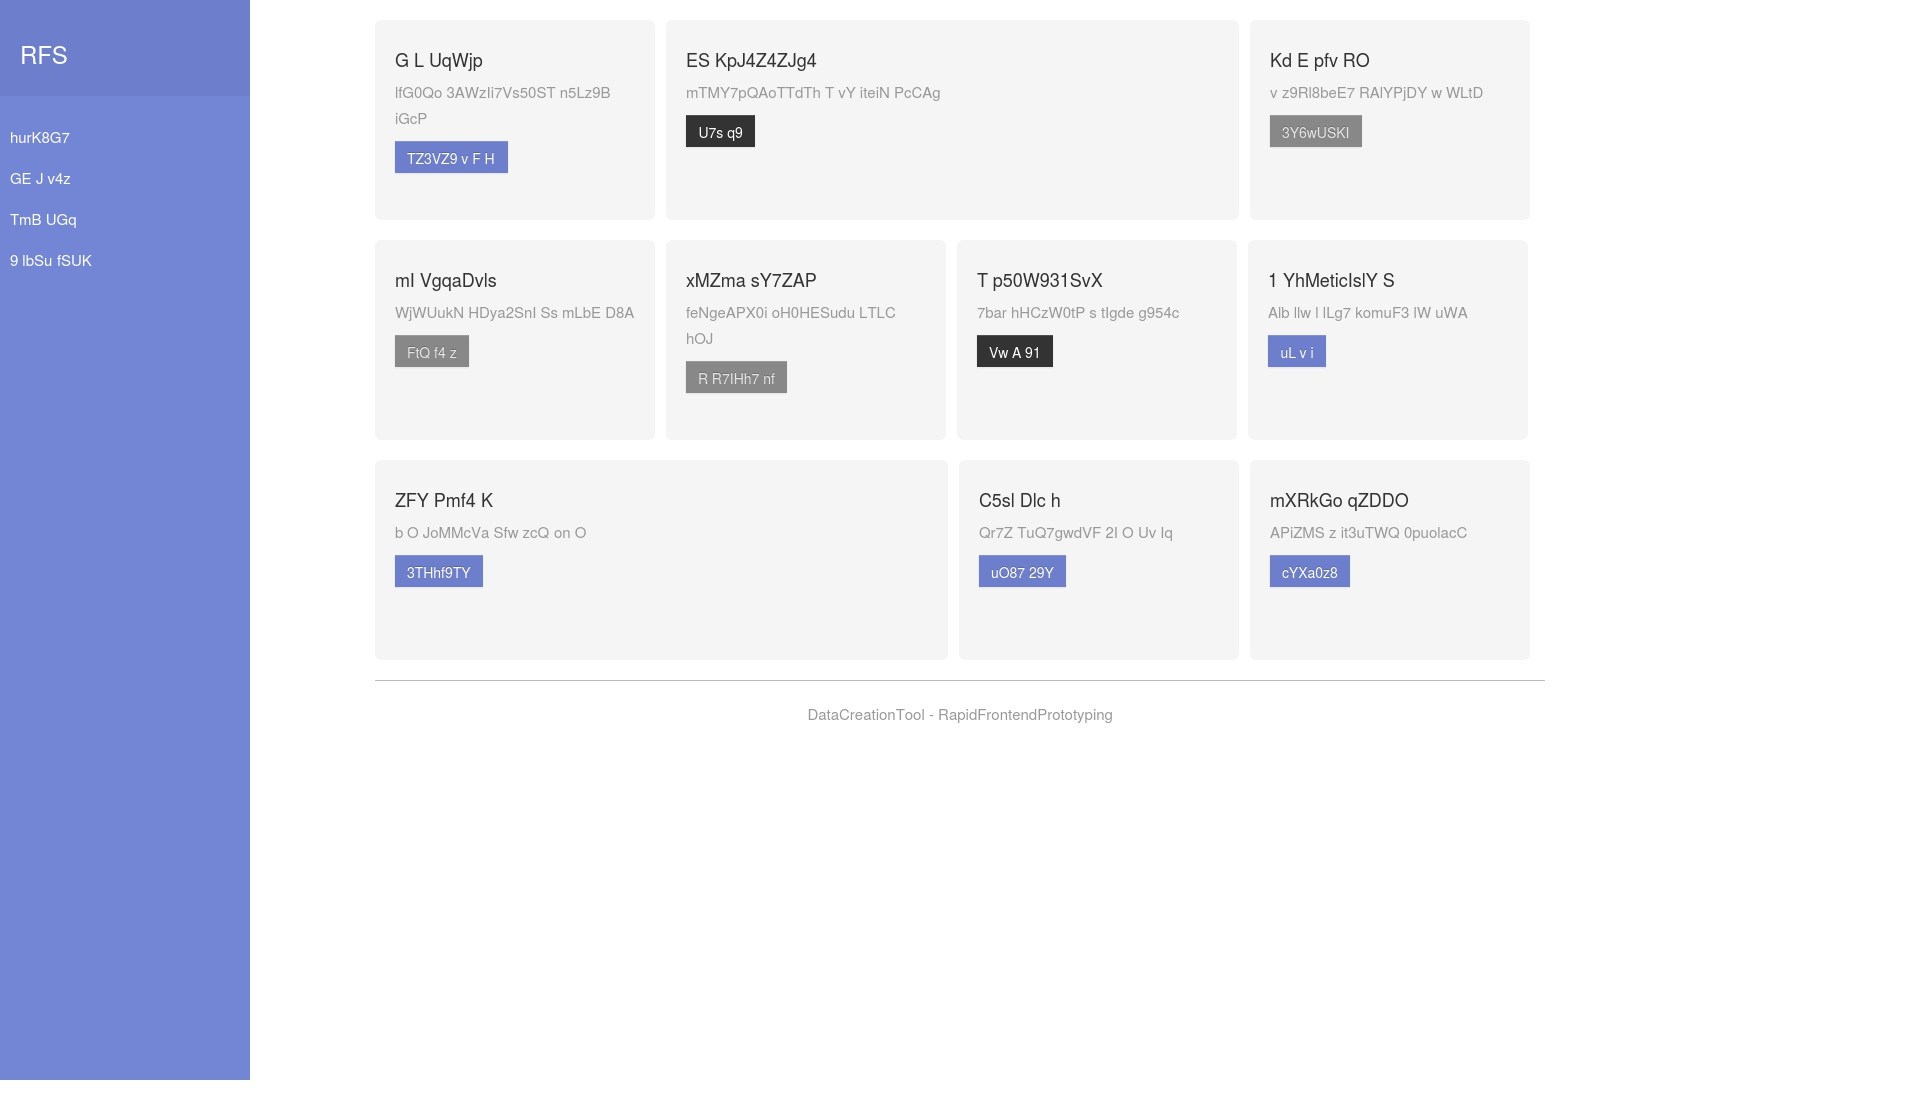
\includegraphics[width=1\textwidth]{beispiel_daten}
\caption{Ein Beispiel Bild aus dem Datenset}
\label{fig:beispiel_daten}
\end{figure}

\subsection{Generieren der Token-Bäume}
Die Token-Bäume werden in der Datei \texttt{dateCreationTool/createAllTokens.py} generiert. Diese Datei erzeugt alle möglichen Token-Kombination anhand der folgenden Regeln:

\subsubsection{Gramatik}

\begin{equation}
start \rightarrow [H,C]
\end{equation}

\begin{equation}
H \rightarrow [Ml | Mr | S]
\end{equation}
\begin{equation}
Ml \rightarrow  [ logoLeft, buttonWhite | logoLeft, buttonWhite, buttonWhite | ...]
\end{equation}
\begin{equation}
Mr \rightarrow [buttonWhite, logoRight | buttonWhite, buttonWhite, logoRight | ...]
\end{equation}
\begin{equation}
S \rightarrow [sidebarHeader, sidebarItem| sidebarHeader, sidebarItem, sidebarItem | ...]
\end{equation}

\begin{equation}
C \rightarrow [R | R, R | R, R, R ]
\end{equation}
\begin{equation}
R \rightarrow [S | D, D, | Q, Q, D | Q, D, Q | D, Q, Q | Q, Q, Q, Q]
\end{equation}
\begin{equation}
S, D, Q \rightarrow [smallTitle, text, contentButton]
\end{equation}
\begin{equation}
contentButton \rightarrow [buttonBlue, buttonGrey, buttonBlack]
\end{equation}

Regeln 3 - 5 sind gekürzt. Es können bis zu 5 Buttons auftreten.

\subsubsection{Zeichenerklärung}

\begin{description}
	\item[H] Header der Website, enthält eins der folgenden Elemente: 
	\begin{description}
		\item[Ml] Menue mit Logo auf der linken Seite
		\item[Mr] Menue mit Logo auf der rechten Seite
		\item[S] Sidebar	
	\end{description}
	\item[C] Content der Website, besteht aus ein bis drei Wiederholungen dieses Elements:
	\begin{description}
		\item[R] Row, die aus einem oder mehreren Row Elementen bestehen kann:
		\begin{description}
			\item[S] Single Row Element, die ganze Row ist mit diesem ausgefüllt.
			\item[D] Double Row Element, ist so breit wie eine Hälfte der Row
			\item[Q] Quadruble Row Element, ist so breit wie ein Viertel der Row
		\end{description}
		Jedes dieser Elemente enthält den gleichen Inhalt:
		\item[smallTitle] Überschrift
		\item[text] Text-Inhalt
		\item[contentButton] Ein Button der entweder Blau, Grau oder Schwarz ist 
	\end{description}
\end{description}

\subsubsection{Token Generierung}

Die Generierung erfolgt mit einfachen, verschachtelten Loops und einem Kartesischen Produkt, um alle möglichen Kombinationen abdecken. Dadurch werden 4128 verschiedene Layout Kombinationen möglich. 
Die Layout-Kombinationen haben eine durchschnittliche Länge von 62.47 Token (Arithmetisches Mittel), bei einen Median von 65 Token. Außerdem ist die mximale Länge 92, die minimale Token Anzahl ist 16.

\begin{verbatim}
    menu_or_sidebar = [True, False]
    logo_left_or_right = [True, False]
    possible_num_of_menu_button = [1, 2, 3, 4]
    possible_num_of_rows = [1,2,3]
    possible_row_type = [0,1,2,3,4]

    row_count_layout_combinations = []

    for i in possible_num_of_rows:
        row_count_layout_combinations.extend( 
            list(itertools.product(possible_row_type, repeat=i))
        )

    for i in range(len(row_count_layout_combinations)):
        row_count_layout_combinations[i] = list(row_count_layout_combinations[i])

    complete_layouts =  []

    for menu_flag in menu_or_sidebar:
        for logo_flag in logo_left_or_right:
            for num_of_menue_button in possible_num_of_menu_button:
                for row_count_layout in row_count_layout_combinations:

                        root = Element("body", "")

                        if menu_flag:
                            menu = tokenBuilder.createMenu(logo_flag, num_of_menue_button)
                            root.addChildren(menu)
                        else:
                            sidebar = tokenBuilder.createSidebar(num_of_menue_button)
                            root.addChildren(sidebar)

                        for i in range(len(row_count_layout)):
                            row = tokenBuilder.createRow(row_count_layout[i])
                            root.addChildren(row)

                        complete_layouts.append(root)
\end{verbatim}

In den ersten fünf Zeilen werden die jeweiligen Konfigurations-Möglichkeiten in Listen geschrieben. Anschließend wird eine weitere Liste erstellt mit allen Möglichen Kombinationen aus Anzahl von Rows und Row Type mit der Funktion itertool.product(). Um dies zu erreichen hätte man auch je nach Anzahl an Rows verschachtelte For-Loops benutzten können, dieser Ansatz wäre jedoch zu unflexibel, falls in Zukunft noch mehr Rows hinzukommen würden.
Als letzter Schritt wird eine Loop pro Liste benutzt um über den gesamten Raum der möglichen Kombinationen zu Iterieren. Dann wird mit der jeweiligen Kombination ein Token-Baum gebildet und der Liste aller Token-Bäume angehängt. Im weiteren Code verlauf wird diese Liste auf mehrerer Threads verteilt und parallel in eigenen Files gespeichert.
Bei der Speicherung wird wie im Fall des Renderings eine rekursive Funktion auf Element-ebene ausgeführt, die den Tag jedes Elements und der Kinder in einen String zusammenführt.

\subsection{DSL Mapping}

Zu jedem dieser Token, existiert ein Mapping nach HTML/CSS. In einer extra Datei, \texttt{dsl-mapping.json} ist dies abgebildet:

\begin{verbatim}
  {
    "opening-tag": "{",
    "closing-tag": "}",
    "body": "<!DOCTYPE html>\n <head>\n <meta charset=\"utf-8\">\n ...
    "header": "<nav class=\"menue\">\n    <ul class=\"nav nav-pills...
    "btn-active": "<li class=\"active\"><a href=\"#\">[]</a></li>\n...
    "btn-inactive-blue": "<button type=\"button\" class=\"btn btn-p...
    "btn-inactive-black": "<button type=\"button\" class=\"btn btn-...
    "btn-inactive-white": "<button type=\"button\" class=\"btn btn-...
    "btn-inactive-grey": "<button type=\"button\" class=\"btn btn-p...
    "row": "<div class=\"container\"><div class=\"row\">{}</div></d...
    "single": "<div class=\"col-lg-12\">\n{}\n</div>\n"
    "double": "<div class=\"col-lg-6\">\n{}\n</div>\n",
    "quadruple": "<div class=\"col-lg-3\">\n{}\n</div>\n",
    "big-title": "<h2>[]</h2>",
    "small-title": "<h4>[]</h4>",
    "text": "<p>[]</p>\n",
    "logo-left": "<a class=\"logo-left\">RFP</a>\n",
    "logo-right": "<a class=\"logo-right\">RFP</a>\n",
    "sidebar": "<div class=\"wrapper\">\n    <div id=\"sidebar\">\...
    "sidebar-element": "<li><a href=\"#\">[]</a><li>"  
  }
  
\end{verbatim}

Um somit aus einem Token-Baum HTML/CSS Markup zu erzeugen, startet der Wurzelknoten eine rekursive Rendering-Funktion. Diese nutzt den zu den Knoten gehörigen Code und traversiert den gesamten Baum. Jeder Mapping String eines Tokens enthält einen Platzhalter, hier \texttt{\{\}}, mit dem signalisiert wird, wo der Code der Kinderknoten hingehört. Ähnlich gibt es ebenso einen Platzhalter für Text-Content, nämlich die Zeichen: \texttt{[]}. 
Für den Text-Content wird im Zuger der Arbeit nur zufällige Zeichenfolgen genommen, damit das Neurale Netzwerk lernt nicht auf den Text zu achten. 


\subsection{Screenshot Erstellung}

Nachdem der HTML/CSS String als Datei abgespeichert wurde, kann mit dem Tool \texttt{imgkit} ein \texttt{.png} oder \texttt{.jpg} erzeugt werden.

\subsection{Teilen der Trainingsdaten}

Die Gesamten Trainingsdaten, werden in ein Trainingsset mit einem Anteil von 70\%, einem Testset mit 20\% und einem Validierungsset mit 10\% der Bilder abgespeichert

\section{Validierung der Ergebnisse}

Um die Qualität der Ergebnisse zu vergleichen, wurde eine Metrik erstellt, welche die Anhand der Wichtigkeit der jeweiligen Elemente einen Score erstellt. Auf Token-Ebene einfach nach Fehlern zu suchen und jeden falschen Token gleich zu gewichten, würde zu nicht aussage-kräftigen Scores leiten. Zum Beispiel ist ein Menü-Item zu viel oder zu wenig, sehr viel weniger schlimm, als eine falsche Kategorisierung des Headers der Website. Um eine ständig gleich bleibende Bewertung der trainierten Netzwerke zu schaffen, ist eine Datei \texttt{evaluateModel.py} implementiert worden. Diese wird nach jedem Trainieren einen Score mit allen Testdaten errechnen. Dazu werden pro Datensatz mehrere Tests gemacht. Der erste Test überprüft ob der Header korrekt ist. Dieser ist einer der am stärksten gewichteten. Danach wird überprüft, ob die Anzahl der Menü-Item korrekt ist. Anschließend wird der Rest des Content geprüft, und zwar die Anzahl an Rows, der richtige Row-Type pro Row und die Anzahl der korrekten sowie falschen Buttons. Pro Datensatz wird so ein \texttt{error\_object} erstellt. 
Hier ein Beispiel:

\begin{verbatim}
{
 'countCorrectButtons': 1,
 'countCorrectRowType': 0,
 'countWrongButtons': 5,
 'countWrongRowType': 3,
 'differenceButtonCount': 3,
 'differenceMenuButtons': 0,
 'differenceRowCount': 0,
 'differenceTokenCount': 16,
 'isHeaderCorrect': True,
 'predictedFileName': './generatedMarkup/second.gui',
 'trueFileName': './generatedMarkup/SECOND_complete_generation_4_04.10.2018_1538655331945.gui',
 'trueHeaderType': 'sidebar',
 'true_token_count': 55
}
\end{verbatim}


Hier hat das Modell insgesamt 16 Tokens zu viel generiert, diese kommen aus zu drei zu viel generierten Buttons, sowie den falschen Row Types. Jede generierte Row hat hier den Falschen Row Type, zu sehen an \texttt{'countCorrectRowType': 0}. Richtig generiert wurde der Header Type, hier wurde die korrekte \texttt{sidebar} verwendet.

Aus diesen Metriken, wird nun folgender Maßen ein Score berechnet:        
\begin{equation}
score = cWB + dBC + dMB + 5 * cWRT + 5 * dRC + iHC * 10
\end{equation}

\begin{description}
	\item[$cWB$] \texttt{countWrongButtons}: Die Anzahl Buttons mit falscher Farbe.
	\item[$dBC$] \texttt{differenceButtonCount}: Der Unterschied in der Anzahl an Buttons.
	\item[$dMB$] \texttt{differenceMenuButtons}: Unterschied der erkannten Menü-Buttons.
	\item[$cWRT$] \texttt{countWrongRowType}: Gibt an wie viele falsche Row-Types gefunden wurden.
	\item[$dRC$] \texttt{differenceRowCount}: Ist die Differenz der Anzahl der Rows.
	\item[$iHC$] \texttt{isHeaderCorrect}: Gibt an ob der Header korrekt ist. Kann entweder den Wert $0$ oder $1$ annehmen.	
\end{description}

Nachdem für jedes Testbild so ein Score berechnet wurde, kann ausgehend von diesem die Performance des Modells genauer bestimmt werden. Um die Verteilung der Scores pro Modell besser verstehen zu können, wird die Verteilung der Fehler anhand mehrerer Lageparameter beschrieben. Dazugehören verschiedene Durchschnitte und Quintile:

  \begin{verbatim}
analysed_scores {
    'median': 6, 
    'mean': 7.47172859450727, 
    'g_mean': 6.192757554950546, 
    'h_mean': 5.272351955758953, 
    'quintiles': {
        'p20': 4,
        'p40': 5, 
        'p60': 7, 
        'p80': 9 
	},
    'most_common_error_count': 5, 
    'count_most_common_error_count': 110
    'count_no_erros': 1, 
}
 \end{verbatim}


Ein weiteres wichtiges Werkzeug hierbei ist ein Histogramm über die Verteilung der Fehlerscores. Bei Vergleich von zwei Histogrammen, Plot~\ref{fig:bsp_plot_good} und Plot~\ref{fig:bsp_plot_bad}, erkennt man, dass bei Plot~\ref{fig:bsp_plot_good} die Anzahl an niedrigen Scores sehr viel höher ist, als bei Plot~\ref{fig:bsp_plot_bad}.

Außerdem findet ein Vergleich der Fehler Typ Verteilungen aller Predictions gegenüber den 20\% schlechtesten Predictions.

\begin{verbatim}
'all': {
    'total_wrong_row_count': 99,
    'total_wrong_headers': 0, 
    'total_count': 619, 
    'total_wrong_row_types': 131, 
    'total_wrong_menue_buttons': 244, 
    'total_wrong_buttons': 2821
    },
'p80': {
    'total_wrong_row_count': 95, 
    'total_wrong_headers': 0, 
    'total_count': 150, 
    'total_wrong_row_types': 128, 
    'total_wrong_menue_buttons': 75, 
    'total_wrong_buttons': 652
    }
\end{verbatim}

\begin{figure}
\centering
\begin{minipage}{.5\textwidth}
  \centering
  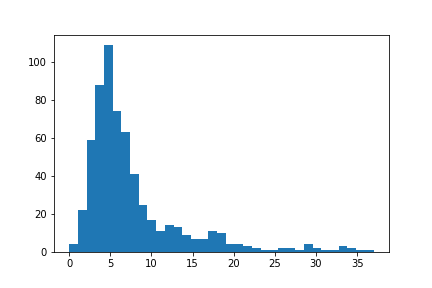
\includegraphics[width=.8\linewidth]{predictions_bin10_histogramm}
  \captionof{figure}{A figure}
  \label{fig:bsp_plot_good}
\end{minipage}%
\begin{minipage}{.5\textwidth}
  \centering
  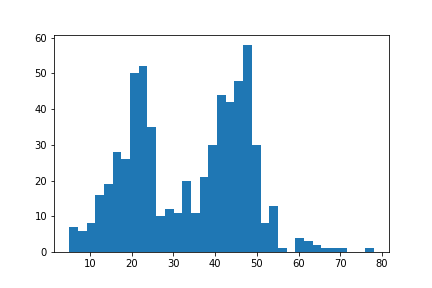
\includegraphics[width=.8\linewidth]{predictions_bin12_histogramm}
  \captionof{figure}{Another figure}
  \label{fig:bsp_plot_bad}
\end{minipage}
\end{figure}

\section{Experimente}

In diesem Abschnitt wird beschrieben, welche Trainingsversuche durchgeführt wurden um ein bestmögliches Ergebnis zu erhalten. Die Beschreibungen für jeden Trainingsversuch sind jeweils in fünf Abschnitte unterteilt. Dazu gehört eine Einführung, das Datenset, eine Auflistung der veränderten Parameter, die Ergebnisse und ein Fazit.

\subsection{Architektur}\label{sub:architektur}
Bevor die Beschreibung der jeweiligen Experimenten beginnt, hier eine Auflistung der Standard Parameter der Modelle. 

\begin{verbatim}
model.summary():
________________________________________________________________________________
Layer (type)                    Output Shape         Param #     Connected to

================================================================================
input_1 (InputLayer)            (None, 256, 256, 3)  0
________________________________________________________________________________
input_2 (InputLayer)            (None, 48, 20)       0
________________________________________________________________________________
sequential_1 (Sequential)       (None, 48, 1024)     104098080   input_1[0][0]
________________________________________________________________________________
sequential_2 (Sequential)       (None, 48, 128)      209920      input_2[0][0]
________________________________________________________________________________
concatenate_1 (Concatenate)     (None, 48, 1152)     0           sequential_1[1][0]
                                                                 sequential_2[1][0]
________________________________________________________________________________
lstm_3 (LSTM)                   (None, 48, 512)      3409920     concatenate_1[0][0]
________________________________________________________________________________
lstm_4 (LSTM)                   (None, 512)          2099200     lstm_3[0][0]
________________________________________________________________________________
dense_3 (Dense)                 (None, 20)           12312       lstm_4[0][0]
================================================================================
\end{verbatim}

Wichtig hierbei sind folgende drei Ebenen des Modells; \texttt{sequential\_1}, \texttt{sequential\_2} und \texttt{concatenate\_1}. 

\begin{description}
	\item[\texttt{sequential\_1}] Dieser Teil ist ein CNN, welches den Screenshot der Website als Input bekommen.
	\item[\texttt{sequential\_2}] Das Sprach Modell, ein rekurrentes Netzwerk, dass die DSL erlernt.
	\item[\texttt{concatenate\_1}] Hier wird der Output des CNN und des Sprach-Modells zusammen geführt und in ein weiteres rekurrentes Netzwerk gegeben welches aus der Sprache und dem Screenshot die Beschreibung dazu findet.
\end{description}

Weitere Hyper-Parameter:
\begin{description}
	\item[Anzahl Netzwerk Paramerter] Insgesamt hat das Netzwerk 109.829.432 trainierbare Parameter und kommt damit auf eine Größe von knapp 420 Mega Byte.
	\item[\texttt{CONTEXT\_LENGTH}] Die \texttt{CONTEXT\_LENGTH} auf 48 Tokens eingestellt. Die \texttt{CONTEXT\_LENGTH} bestimmt die Größe des Sliding-Windows, mit dem die Input Token Sequenzen abgearbeitet werden. 
	\item[\texttt{IMAGE\_SIZE}] Die Größe der Input Bilder ist 256 mal 256 Pixel.
	\item[\texttt{BATCH\_SIZE}] Trainiert wird in Batches mit jeweils 64 Bildern
	\item[\texttt{EPOCHS}] Es werden 10 Epochen trainiert.
	\item[\texttt{STEPS\_PER\_EPOCH}] In jeder Epoche weren 72.000 Schritte gemacht.
	
\end{description}

\subsection{Training}\label{sub:training}

Da es für jeden Screenshot eine zugehörige Token-Sequenz mit variabler Länge gibt, müssen die Trainingsdaten mit einem Sliding-Window-Prinzip abgearbeitet werden. Dafür werden aus der Token-Sequenz, $n$ Samples gebildet, wobei $n = len(token\_sequence) - CONTEXT\_LENGTH$. Das Modell bekommt pro Screenshot $n$ Paare aus Screenshot und dazugehörigen Token-Kontext. Wichtig hierbei ist, dem Modell mitzuteilen, wann eine Sequenz beginnt und wieder endet, dafür gibt es einen \texttt{start}-Token sowie einen \texttt{end}-Token. Diese werden je als pre- bzw. suffix an die Token-Sequenz angefügt bevor die $n$ Samples gebaut werden. 

So kann während dem Training mit Backpropagation ein klassischer Multi-Class-Loss optimiert werden.
\begin{equation}
L(I, X) =  -\sum_{t=1}^T x_{t+1} log(y_t)
\end{equation}

Hierbei ist $x_{t+1}$ der erwartete Token und $y_t$ der berechnete. Das Modell ist in einer Gesamtheit ableitbar, dies bedeutet, der CNN-Teil kann zusammen mit den beiden LSTMs optimiert werden. Wie im Original Paper, wurde mit RMSProp-Algorithmus trainiert, mit einer Learning Rate von $0,0001$. Außerdem wurden die Gradienten um die numerische Stabilität zu erhöhen, werden die Output Gradienten in das Intervall $[-1,1]$ getrimmt. Es wird eine Dropout-Regulation genutzt als eine Maßnahme gegen Overfitting. Im CNN nach den Max-Pooling Ebenen mit 25\% und nach den Fully-Connected Ebenen mit 30\%.


\subsection{1. Trainingsversuch}

\subsubsection*{Einführung}

Um eine Baseline aller weiteren Ergebnisse zu erstellen, wird das Original Modell aus dem pix2code Paper mit meinen neuen Daten neu trainiert. 

\subsubsection*{Datenset}

Das verwendete Datenset enthält 4128 Bilder, von denen 2890 für das Training verwendet werden. Die, das Datenset beschreibende, DSL enthält 24 Token. Jedes Bild wird mit durchschnittlich 62,47 Token (Median: 65) beschrieben, die maximale Anzahl liegt bei 92 Token, die minimale Anzahl bei 16. 

\subsubsection*{Veränderte Parameter}

Für diese Baseline wurden alle Parameter unverändert übernommen. Die einzige Anpassung die gemacht werden mussen, sind zwei Ebenen im Netzwerk, dessen Input und Output die Anzahl der Token reflektieren. Dies sind Ebene \texttt{input\_2} und \texttt{dense\_3}. Der Shape der beiden Ebenen wurde angepasst um mit 24 Token arbeiten zu können. Daher ist dieser in der Input-Ebene \texttt{(None, 48, 24)} anstatt \texttt{(None, 48, 20)}. Ebense bei der Dense-Ebene \texttt{(None, 24)} anstatt \texttt{(None, 20)}.

\subsubsection*{Ergebnis}

Nach dem Training des Netzwerkes wurden mehrere zufällige Bilder ($n=10$) aus dem Test Set ausgewertet. Bei jedem einzelnen der Bilder kommt das selbe Ergebnis:

\begin{verbatim}
body {
	sidebar {
		sidebar-element,sidebar-element,sidebar-element,sidebar-element
	},
	row {
		quadruple {
			small-title,text,btn-inactive-blue
		},
		quadruple {
			small-title,text,btn-inactive-blue
		},
		double {
			small-title,text,btn-inactive-blue
		}
	},
	row {
		quadruple {
			small-title,text,btn-inactive-blue
		},
		quadruple {
			small-title,text,btn-inactive-blue
		},
		double {
			small-title,text,btn-inactive-blue
		}
	},
	row {
		quadruple {
			small-title,text,btn-inactive-blue
		},
		quadruple {
			small-title,text,btn-inactive-blue
		},
		double {
			small-title,text,btn-inactive-blue
		}
}
\end{verbatim}

\subsubsection*{Fazit}

Anhand des Ergebnisses kann man sagen, dass entweder die erhöhte Token Anzahl, oder die neuen Trainingsbilder, zu viel Entropie in die Trainingsdaten bringen. So kann das Modell leider zu keinem sinnvollen Optimum konvergieren. 


\subsection{2. Trainingsversuch}

\subsubsection*{Einführung}

In diesem Versuch wurde eine vergrößerte Context-Länge erprobt. Da im ersten Versuch, das Training nicht funktioniert hat, vermute ich den Fehler in einem zu kleinen Sichtbereich des LSTMs. Da durch die Token-Länge die Sichtbarkeit der Long-Term-Dependencies geregelt wird, verdoppel ich diese um zu sehen, ob dadurch ein verbessertes Ergebnis zustande kommt.

\subsubsection*{Datenset}

Gleichbleibend zum ersten Versuch.

\subsubsection*{Veränderte Parameter}

Das Modell ist genau gleich wie im ersten Versuch, lediglich die Context-Länge wurde von 48 auf 96 erhöht.

\subsubsection*{Ergebnis}

Wie bei ersten Versuch ergibt dieses Training wieder den gleichen Output. Egal welches Bild als Input genommen wird. Um sicher zu gehen, dass diese Prediction nicht zufällig von dem gewählten Testbild abhängt, habe ich insgesamt 313 Bilder getestet, um festzustellen, das alle diese Bilder zum gleichen Ergebnis führen. Alle dieser Bilder bekommen den exakt gleichen Output

\subsubsection*{Fazit}

An einem zu geringen Kontext kann das nicht konvergierende Training nicht liegen. In den folgenden Versuchen werden andere Parameter verändert.

\subsection{3. Trainingsversuch}


\subsubsection*{Einführung}

Da im ersten und zweiten Versuch, mit der Original Architektur kein brauchbares Ergebnis herausgekommen ist, und das Netz ein zu falsches Ergebnis liefert, wird nun versucht mit einer höheren Komplexität der LSTMs ein Modell zu finden das besser funktioniert.

\subsubsection*{Datenset}

Gleichbleibend zum ersten Versuch.

\subsubsection*{Veränderte Parameter}

Hier hab ich die Anzahl der LSTM \texttt{units} von 128, im Language Modell, auf 192 erhöht. Außerdem erfolgte eine Veränderung der LSTM \texttt{units} von 512 auf 768 im Decoder Modell.

\begin{verbatim}
________________________________________________________________________________
Layer (type)                    Output Shape         Param #     Connected to
================================================================================
input_1 (InputLayer)            (None, 256, 256, 3)  0
________________________________________________________________________________
input_2 (InputLayer)            (None, 48, 24)       0
________________________________________________________________________________
sequential_3 (Sequential)       (None, 48, 1024)     104098080   input_1[0][0]
________________________________________________________________________________
sequential_4 (Sequential)       (None, 48, 192)      462336      input_2[0][0]
________________________________________________________________________________
concatenate_1 (Concatenate)     (None, 48, 1216)     0           sequential_3[1][0]
                                                                 sequential_4[1][0]
________________________________________________________________________________
lstm_3 (LSTM)                   (None, 48, 768)      6097920     concatenate_1[0][0]
________________________________________________________________________________
lstm_4 (LSTM)                   (None, 768)          4721664     lstm_3[0][0]
________________________________________________________________________________
dense_3 (Dense)                 (None, 24)           18456       lstm_4[0][0]
================================================================================
Total params: 115,398,456
Trainable params: 115,398,456
Non-trainable params: 0

________________________________________________________________________________
\end{verbatim}

Durch diese Veränderung gibt es ca. 8 Millionen mehr Parameter.
Die Länge des Kontextes wurde zurück auf 48 gestellt.

\subsubsection*{Ergebnis}

Exakt gleiches Ergebnis zu den beiden ersten Versuchen.

\subsubsection*{Fazit}

Da inzwischen immer noch der gleiche Output generiert wird, probiere ich nun einen Fehler im Programm-Code zu finden. Folgende Ursachen könnte es geben:

\begin{description}
	\item[Fehler im Sampler] Der Sampler generiert nach dem Training aus Screenshots die Token-Sequenz. Hier könnte zum einen, ein falsches Modell geladen werden, oder es wird fehlerhaft geladen.
	
	\begin{description}
		\item[Falsches Modell] Durch Umbenennung des Modells im Output Folder und Eingabe eines falschen Modellnamens, bricht das Programm jeweils ab.
		\item[Fehlerhaftes Laden] Die Ausgabe von \texttt{model.summary()} nach dem Laden des Modells ist identisch mit der erstellten während des Trainings.
	\end{description}
	
	\item[Fehler in den Daten] Während dem Preprocessing werden die Trainingsbilder in \texttt{numpy}-Arrays mit \texttt{shape(256,256,3} umgewandelt. Anschließend werden die Arrays und \texttt{gui}-Files zusammen abgespeichert.
	
	\begin{description}
		\item[Array Konvertierung] Beweis Bild + Nach optischer Kontrolle von zufälligen Samples ($n=10$) musste ich feststellen, dass diese korrekt sind.
		\item[Zuordnung Files] Nach Kontrolle zufälliger Samples sieht die Zuordnung ebenfalls gut aus.
	\end{description}
	
	\item[Fehler in Vocabulary] Es könnte auch an der fehlerhaften Abspeicherung der einzelnen Tokens liegen. Vocabulary und One-Hot-Encoding sind ebenfalls richtig.
	
	\item[Fehler im Datenset / -synthese] Hier wurde ein Fehler gefunden: Alle Screenshots, welche die \texttt{sidebar} anstatt des \texttt{menue} haben, sind doppelt enthalten. Der Grund hierfür ist die Positionierung des Menü-Logos. Da es in Falle des \texttt{menue} zwei Möglichkeiten für die Positionierung des Logos gibt, wurden diese durch iteriert in der Erstellung der Daten. Da es bei der \texttt{sidebar} diese beiden Möglichkeiten aber nicht gab, wurden so alle Bilder mit der \texttt{sidebar} doppelt erstellt. Ein Viertel der Trainingsdaten hat ein Menü mit Logo links, ein weiteres Viertel hat das Logo rechts. Die andere Hälfte der Trainingsdaten hat die \texttt{sidebar}, in denen aber nur halb so viele einmalige enthalten sind.
	
\end{description}

\subsection{4. Trainingsversuch}


\subsubsection*{Einführung}

Nach dem Finden des Fehlers im vorherigen Versuch, wurde ein neues Datenset erstellt.

\subsubsection*{Datenset}

Ei neues Datenset mit 3096 Bildern wurde erstell. Ein Drittel hat das Feature \texttt{menue\_logo\_left}, ein Drittel \texttt{menue\_logo\_right}, und der Rest die \texttt{sidebar}. 

\subsubsection*{Veränderte Parameter}

In diesem Versuch wurden die gleichen Parameter wie im ersten Versuch genutzt.

\subsubsection*{Ergebnis}

Es erfolgte keine Verbesserung der Trainingsergebnisse. Die Token-Sequenz hat sich dahingehend geändert, dass nun anstatt der \texttt{sidebar} ein Menü in allen Ergebnissen ist.

\begin{verbatim}
body{
header{
logo-right,btn-inactive-white,btn-inactive-white
}
row{
quadruple{
small-titletextbtn-inactive-black
}
quadruple{
small-titletextbtn-inactive-black
}
double{
small-titletextbtn-inactive-black
}
}
row{
quadruple{
small-titletextbtn-inactive-black
}
quadruple{
small-titletextbtn-inactive-black
}
double{
small-titletextbtn-inactive-black
}
}
}
\end{verbatim}

\subsubsection*{Fazit}

Die gefundene Token Sequenz muss wohl die allgemeingültigste sein, da diese immer wieder gefunden wird. Da der Fehler nicht an einem Fehler im Programm liegt, muss er entweder in den Daten oder im Modell liegen. 

\subsection{5. Trainingsversuch}

\subsubsection*{Einführung}

Gleichzeitig zu dem 4. Versuch wurde noch ein Subset der Daten erstellt, das nur 70\% der Bilder aufweist. Dieses hat 2166 Bilder im Vergleich zu dem Set vom 4. Trainingsversuch. Der Gedanke hierbei ist, dass im Original Training vom pix2code Paper 1500 Trainingsbilder ausgereicht haben. Unter Umständen konvergiert es mit weniger Daten zu einem anderen Durchschnittswert oder fängt an die richtigen Ergebnisse herauszufinden.

\subsubsection*{Datenset}
Eine reduzierte Variante des Sets aus dem vierten Versuch.

\subsubsection*{Veränderte Parameter}

Gleiche Parameter wie im ersten Versuch.
%bin8

\subsubsection*{Ergebnis}

Es erfolgte keine Verbesserung der Trainingsergebnisse.

\subsubsection*{Fazit}

Dieser Ansatz hat gezeigt, dass dieser Weg der falsche ist.

\subsection{6. Trainingsversuch}

\subsubsection*{Einführung}

Nach Analyse der Daten des Original Papers, wurde festgestellt, dass dort ein Tag weggelassen wurde. Es wird kein \texttt{body}-Tag verwendet. Dieser ist bei jedem der Bild-beschreibenden Token-Sequenzen der root-Knoten. Da er jedes mal auftritt, hat er aber keine Relevanz zu dem Screenshot und kann daher weggelassen werden.

\begin{verbatim}
python train.py ../../data/rfp_data_no_body_3096_11.10.
2018/train/ ../bin9/ 1

\end{verbatim}

\subsubsection*{Datenset}

Neues Datenset, ohne \texttt{body}-Tags. Dieses hat insgesamt 3096 Bilder und ist wieder 70-20-10 gesplittet in Trainings-, Test- und Validierungsset. Durch das Fehlen des \texttt{body}-Tags ergibt sich folgende Verteilungsmaße:
\begin{verbatim}
Token length analysis:
     mean token length:    59.69
     max token length:     89
     min token length:     14
     median token length:  62
\end{verbatim}

Die Median-Token-Länge ist um genau 3 Token geringer geworden. Dies liegt daran, dass zugehörig zum \texttt{body}-Tag zwei Klammern benötigt wurden (\texttt{\{} und \texttt{\}}), welche anzeigen, dass der Rest der Token Kinds-Knoten des \texttt{body}-Tags sind.

\subsubsection*{Veränderte Parameter}

Gleiche Parameter wie im ersten Versuch.

\subsubsection*{Ergebnis}

Es kommt die gleiche Ergebnis-Sequenz wie bei den Versuchen davor heraus.

\begin{verbatim}

header{
logo-right,btn-inactive-white,btn-inactive-white
}
row{
quadruple{
small-title,text,btn-inactive-black
}
quadruple{
small-title,text,btn-inactive-black
}
double{
small-title,text,btn-inactive-black
}
}
row{
quadruple{
small-title,text,btn-inactive-black
}
quadruple{
small-title,text,btn-inactive-black
}
double{
small-title,text,btn-inactive-black
}
}

\end{verbatim}

Diesmal jedoch ohne \texttt{body}-Tag.


\subsubsection*{Fazit}

Das Scheitern des Trainings wurde nicht durch die Verkleinerung der DSL behoben. Als nächster Schritt sollte jeweils der Sprach- sowie das Bild-Teil des Modells näher in Betracht genommen werden. Ein Großteil der Parameter des Modells sind bereits im CNN (hier erfolgt die Analyse des Bildes), deswegen wird es die Gesamtperformance weniger stark verbessern, wenn man die gleiche Zahl an neuen Parametern hier hinzufügt. Deswegen wird zunächst der Sprach- und der Decoder-Teil des Modell untersucht.

\subsection{7. Trainingsversuch}

%Versuch mit GRUs \cite{GRUvsLSTM} \cite{lstmSearchSpace}
%bin10

\subsubsection*{Einführung}

Wie im Fazit des vorangegangen Versuchs, wird nun daran gearbeitet, die LSTMs, welche der sprach analysierende und der decodierende Teil des Modells sind zu verbessern. Nach der Lektüre eines Posts von Colahs Blog, wurden testweise die klassischen LSTMs durch GRUs ersetzt.

\subsubsection*{Datenset}

Hier wurde das Datenset aus dem sechsten Trainingsversuch verwendet.

\subsubsection*{Veränderte Parameter}

\begin{verbatim}
________________________________________________________________________________
Layer (type)                    Output Shape         Param #     Connected to
================================================================================
input_1 (InputLayer)            (None, 256, 256, 3)  0
________________________________________________________________________________
input_2 (InputLayer)            (None, 48, 23)       0
________________________________________________________________________________
sequential_1 (Sequential)       (None, 48, 1024)     104098080   input_1[0][0]
________________________________________________________________________________
sequential_2 (Sequential)       (None, 48, 128)      157056      input_2[0][0]
________________________________________________________________________________
concatenate_1 (Concatenate)     (None, 48, 1152)     0           sequential_1[1][0]
                                                                 sequential_2[1][0]
________________________________________________________________________________
gru_3 (GRU)                     (None, 48, 512)      2557440     concatenate_1[0][0]
________________________________________________________________________________
gru_4 (GRU)                     (None, 512)          1574400     gru_3[0][0]
________________________________________________________________________________
dense_3 (Dense)                 (None, 23)           11799       gru_4[0][0]
================================================================================

Trainable params: 108,398,775

\end{verbatim}

Die LSTMs in \texttt{sequential\_2} sowie in Ebene 3 und 4 wurden durch GRUs ersetzt. Die Anzahl der \texttt{units} wurde beibehalten (128 bzw. 512). Dadurch, dass im GRU die Input- und Forget-Gates gekoppelt sind, hat das Modell jetzt eine Millionen Parameter weniger.

\subsubsection*{Ergebnis}

Anstatt der bereits mehrmals auftretenden Token Abfolge, gelingt es diesem Modell richtige Predictions zu erstellten. Alle der 619 getesteten Files konnten ohne Fehler compiliert werden. Die Analyse der Fehlerverteilung ergibt folgende Lageparameter in Abbildung~\ref{fig:lage_bin10}. Die Verteilung der Fehleranzahlen ist in Abbildung~\ref{fig:hist_bin10} gegeben.



\begin{figure}
\centering
\begin{minipage}{.5\textwidth}
  \centering
  \begin{description}
	\item[Arithmetisches Mittel] $7.82$	
	\item[Geometrisches Mittel] $6.36$
	\item[Harmonisches Mittel] $5.34$
	\item[Quintile] p20: $4$, p40: $5$, p60: $7$, p80: $10$
	\item[Median] $6$
	\item[Modus] $5$
	\item[Vorkommen Modus] $109$
	\item[Gesamt Fehler Score] 4840
	\item[Anzahl Token Testset] 36751 
	\item[Anzahl generierter Token] 36186
	\item[Score pro Token in Testset] 0.1317
\end{description}
  \captionof{figure}{Lageparameter}
  \label{fig:lage_bin10}
\end{minipage}%
\begin{minipage}{.5\textwidth}
  \centering
  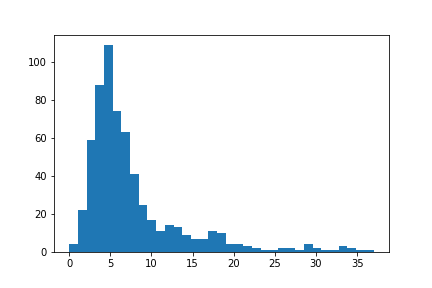
\includegraphics[width=1\linewidth]{predictions_bin10_histogramm}
  \captionof{figure}{Fehlerverteilung}
  \label{fig:hist_bin10}
\end{minipage}
\end{figure}



\begin{comment}
\begin{figure}
\centering
\begin{minipage}{.5\textwidth}
  \centering
  \begin{description}
	\item[Arithmetisches Mittel] $13.98$	
	\item[Geometrisches Mittel] $11.33$
	\item[Harmonisches Mittel] $8.73$
	\item[Quintile] p20: $6$, p40: $9$, p60: $16$, p80: $23$
	\item[Median] $12$
	\item[Modus] $7$
	\item[Vorkommen Modus] $46$
	\item[Gesamt Fehler Score]
	\item[Anzahl generierter Token]
	\item[Score pro Token]
\end{description}
  \captionof{figure}{Lageparameter}
  \label{fig:lage_bin12}
\end{minipage}%
\begin{minipage}{.5\textwidth}
  \centering
  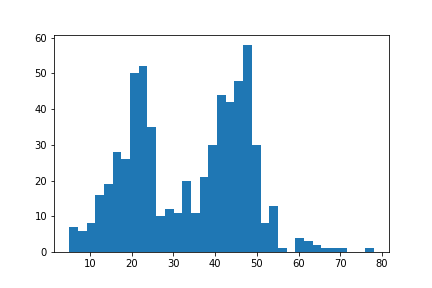
\includegraphics[width=1\linewidth]{predictions_bin12_histogramm}
  \captionof{figure}{Fehlerverteilung}
  \label{fig:hist_bin12}
\end{minipage}
\end{figure}
\end{comment}

Im Weiteren wird das letzte Quintil der Fehler analysiert und mit dem Rest verglichen. In der Abbildung~\ref{fig:fehler_gesamt_bin10} ist die Fehlerverteilung aller Testdaten zusehen, in Abbildung~\ref{fig:fehler_beste80_bin10} die besten 80\% und in Abbildung~\ref{fig:fehler_schlechteste20_bin10} die schlechtesten 20\%. 

\begin{figure}
\centering
\begin{minipage}{.5\textwidth}
  \centering
  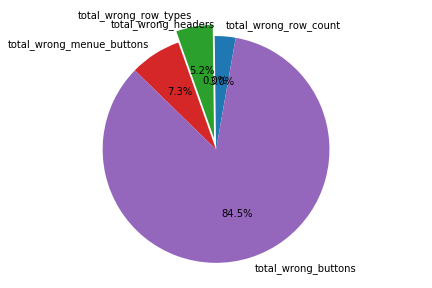
\includegraphics[width=1\linewidth]{predictions_bin10_total_error_types_pie_chart}
  \captionof{figure}{Gesamt}
  \label{fig:fehler_gesamt_bin10}
\end{minipage}%
\begin{minipage}{.5\textwidth}
  \centering
  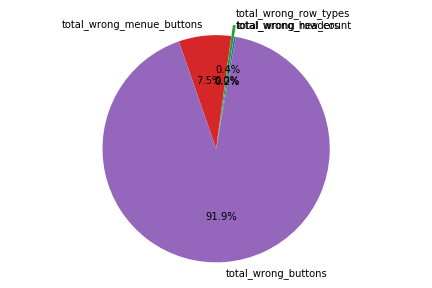
\includegraphics[width=1\linewidth]{predictions_bin10_excluded_p80_error_types_pie_chart}
  \captionof{figure}{Ohne p80}
  \label{fig:fehler_beste80_bin10}
\end{minipage}
\begin{minipage}{.5\textwidth}
  \centering
   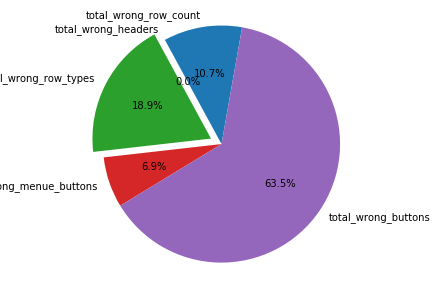
\includegraphics[width=1\linewidth]{predictions_bin10_p80_error_types_pie_chart}
  \captionof{figure}{Nur p80}
  \label{fig:fehler_schlechteste20_bin10}
\end{minipage}%
\end{figure}

Bei 80\% aller Testdaten sind die Fehleruhrsachen zu 92\% ausschließlich falsche Buttons! Außerdem ist die Verteilung der Row Types über den Testdaten sehr genau, wie in Abbildung~\ref{fig:bin10_row_type} zu sehen ist. Mit einer Perfekten Prediction müsste jeder Row Type mit $16,\frac{2}{3}\%$ vorliegen.

\begin{figure}[h]
\centering
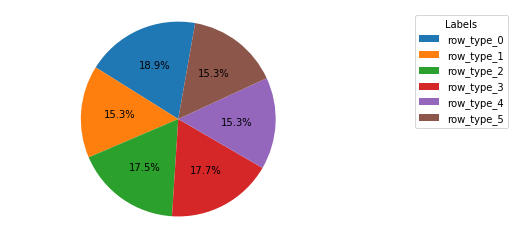
\includegraphics[width=0.5\textwidth]{predictions_bin10_predicted_row_type_distribution}
\caption{Verteilung Row Types}
\label{fig:bin10_row_type}
\end{figure}


\subsubsection*{Fazit}

Dieses Training war ein voller Erfolg. Es ergibt eine hohe Testgenauigkeit und es hat weniger Parameter als das Original Modell aus dem Paper. 

\begin{comment}
4010/4009 [==============================] - 1565s 390ms/step - loss: 0.3897
Epoch 2/10
4010/4009 [==============================] - 1555s 388ms/step - loss: 0.1842
Epoch 3/10
4010/4009 [==============================] - 1555s 388ms/step - loss: 0.1669
Epoch 4/10
4010/4009 [==============================] - 1546s 386ms/step - loss: 0.1543
Epoch 5/10
4010/4009 [==============================] - 1528s 381ms/step - loss: 0.1442
Epoch 6/10
4010/4009 [==============================] - 1528s 381ms/step - loss: 0.1331
Epoch 7/10
4010/4009 [==============================] - 1528s 381ms/step - loss: 0.1240
Epoch 8/10
4010/4009 [==============================] - 1530s 381ms/step - loss: 0.1191
Epoch 9/10
4010/4009 [==============================] - 1529s 381ms/step - loss: 0.1157
Epoch 10/10
4010/4009 [==============================] - 1528s 381ms/step - loss: 0.1135
\end{comment}

\subsection{8. Trainingsversuch}

%language modell: LSTM
%Decoder: GRU
%bin11


\subsubsection*{Einführung}

In diesem Versuch wird eine Kombination aus der Original Architektur mit LSTMs und der neuen mit GRUs aus dem siebten Trainingsversuch getestet. Das Sprach-Modell wird wie im Original mit LSTMs gebildet, der Decoder hingegen mit den GRUs. 

\subsubsection*{Datenset}

Hier wurde das Datenset aus dem sechsten Trainingsversuch verwendet.

\subsubsection*{Veränderte Parameter}

Wie folgt wurde das Modell verändert:
\begin{verbatim}

Layer (type)                    Output Shape         Param #     Connected to
================================================================================
input_1 (InputLayer)            (None, 256, 256, 3)  0
________________________________________________________________________________
input_2 (InputLayer)            (None, 48, 23)       0
________________________________________________________________________________
sequential_1 (Sequential)       (None, 48, 1024)     104098080   input_1[0][0]
________________________________________________________________________________
sequential_2 (Sequential)       (None, 48, 128)      209408      input_2[0][0]
________________________________________________________________________________
concatenate_1 (Concatenate)     (None, 48, 1152)     0           sequential_1[1][0]
                                                                 sequential_2[1][0]
________________________________________________________________________________
gru_1 (GRU)                     (None, 48, 512)      2557440     concatenate_1[0][0]
________________________________________________________________________________
gru_2 (GRU)                     (None, 512)          1574400     gru_1[0][0]
________________________________________________________________________________
dense_3 (Dense)                 (None, 23)           11799       gru_2[0][0]
================================================================================

Trainable params: 108,451,127

\end{verbatim}

Die Ebene \texttt{sequential\_2} ist durch ein LSTM realisiert, die Ebenen \texttt{gru\_1} und \texttt{gru\_2} jeweils durch ein GRU. 

\subsubsection*{Ergebnis}

Jeder der getesteten Daten erzeugt den selben Output:
\begin{verbatim}
header{
logo-right,btn-inactive-white,btn-inactive-white
}
row{
quadruple{
small-title,text,btn-inactive-black
}
quadruple{
small-title,text,btn-inactive-black
}
double{
small-title,text,btn-inactive-black
}
}
row{
quadruple{
small-title,text,btn-inactive-black
}
quadruple{
small-title,text,btn-inactive-black
}
double{
small-title,text,btn-inactive-black
}
}
\end{verbatim}

\subsubsection*{Fazit}

Dieses Ergebnis legt Nahe, dass das Bottleneck des Modells in dem Sprach-Modell liegt. 

\subsection{9. Trainingsversuch}


%language modell: GRU
%Decoder: LSTM
\begin{comment}
python train.py ../../data/rfp_data_no_body_3096_11.10.
2018/train/ ../bin12/ 1

4010/4009 [==============================] - 1646s 410ms/step - loss: 0.5490
Epoch 2/10
4010/4009 [==============================] - 1643s 410ms/step - loss: 0.1962
Epoch 3/10
4010/4009 [==============================] - 1642s 410ms/step - loss: 0.1932
Epoch 4/10
4010/4009 [==============================] - 1642s 410ms/step - loss: 0.1920
Epoch 5/10
4010/4009 [==============================] - 1632s 407ms/step - loss: 0.1916
Epoch 6/10
4010/4009 [==============================] - 1615s 403ms/step - loss: 0.1917
Epoch 7/10
4010/4009 [==============================] - 1616s 403ms/step - loss: 0.1940
Epoch 8/10
4010/4009 [==============================] - 1616s 403ms/step - loss: 0.1869
Epoch 9/10
4010/4009 [==============================] - 1616s 403ms/step - loss: 0.1854
Epoch 10/10
4010/4009 [==============================] - 1609s 401ms/step - loss: 0.1783
\end{comment}


\subsubsection*{Einführung}

Nach dem Testen, ob es reicht allein den Decoder durch ein GRU zu ersetzten, um das Modell konvergieren zu lassen, wird nun das Gegenteil getestet: Ob es auch ausreichend wäre, das Sprach-Modell mit GRUs zu realisieren.

\subsubsection*{Datenset}

Hier wurde das Datenset aus dem sechsten Trainingsversuch verwendet.

\subsubsection*{Veränderte Parameter}

Wie bereits in dem Original Paper, ist hier der Decoder mit LSTMs realisiert, zusehen in den Ebenen \texttt{lstm\_1} und \texttt{lstm\_1}. Die Ebene \texttt{sequential\_2} ist wie im erfolgreichen siebten Trainingsversuch ein GRU.

\begin{verbatim}
Layer (type)                    Output Shape         Param #     Connected to
===============================================================================
input_1 (InputLayer)            (None, 256, 256, 3)  0
_______________________________________________________________________________
input_2 (InputLayer)            (None, 48, 23)       0
_______________________________________________________________________________
sequential_1 (Sequential)       (None, 48, 1024)     104098080   input_1[0][0]
_______________________________________________________________________________
sequential_2 (Sequential)       (None, 48, 128)      157056      input_2[0][0]
_______________________________________________________________________________
concatenate_1 (Concatenate)     (None, 48, 1152)     0           sequential_1[1][0]
                                                                 sequential_2[1][0]
_______________________________________________________________________________
lstm_1 (LSTM)                   (None, 48, 512)      3409920     concatenate_1[0][0]
_______________________________________________________________________________
lstm_2 (LSTM)                   (None, 512)          2099200     lstm_1[0][0]
_______________________________________________________________________________
dense_3 (Dense)                 (None, 23)           11799       lstm_2[0][0]
===============================================================================

Trainable params: 109,776,055

\end{verbatim}

Durch das Benutzen von LSTMs im Decoder, ist die Anzahl der Parameter wieder auf knappe 110 Millionen gewachsen.

\subsubsection*{Ergebnis}

Ähnlich wie das siebte Training konnte das Netzwerk konvergieren und einen nicht allgemeinen Output erzeugen. Die Analyse der Testdaten zeigte jedoch, dass insgesamt 143 der 619 Daten nicht kompiliert werden konnten. 

Die Analyse der Fehlerverteilung ergibt folgende Lageparameter in Abbildung~\ref{fig:lage_bin12}. Die Verteilung der Fehler-Scores ist in Abbildung~\ref{fig:hist_bin12} gegeben.

\begin{figure}
\centering
\begin{minipage}{.5\textwidth}
  \centering
  \begin{description}
	\item[Arithmetisches Mittel] $33.50$	
	\item[Geometrisches Mittel] $30.23$
	\item[Harmonisches Mittel] $26.45$
	\item[Quintile] p20: $20$, p40: $26$, p60: $41$, p80: $46$
	\item[Median] $36$
	\item[Modus] $46$
	\item[Vorkommen Modus] $32$
	\item[Gesamt Fehler Score] 20734
	\item[Anzahl Token Testset] 36751 
	\item[Anzahl generierter Token] 49012
	\item[Score pro Token in Testset] 0.56
\end{description}
  \captionof{figure}{Lageparameter}
  \label{fig:lage_bin12}
\end{minipage}%
\begin{minipage}{.5\textwidth}
  \centering
  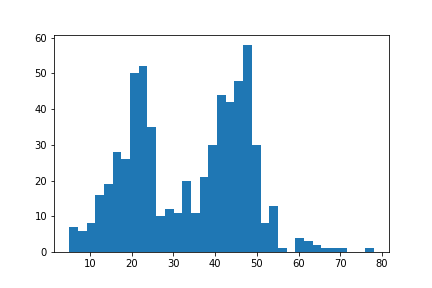
\includegraphics[width=1\linewidth]{predictions_bin12_histogramm}
  \captionof{figure}{Fehlerverteilung}
  \label{fig:hist_bin12}
\end{minipage}
\end{figure}

Der Vergleich zu den Lageparametern~\ref{fig:lage_bin10} des siebten Experiment, performt dieses Modell sehr viel schlechter. Die Median Fehler-Score dieses Experiments ist fünfmal so hoch wie die des siebtens.

Im Weiteren wird das letzte Quintil der Fehler analysiert und mit dem Rest verglichen. In der Abbildung~\ref{fig:fehler_gesamt_bin12} ist die Fehlerverteilung aller Testdaten zusehen, in Abbildung~\ref{fig:fehler_beste80_bin12} die besten 80\% und in Abbildung~\ref{fig:fehler_schlechteste20_bin12} die schlechtesten 20\%. 

\begin{figure}
\centering
\begin{minipage}{.5\textwidth}
  \centering
  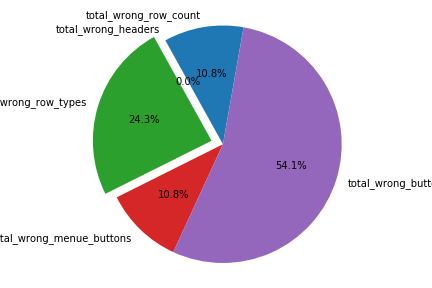
\includegraphics[width=1\linewidth]{predictions_bin12_total_error_types_pie_chart}
  \captionof{figure}{Gesamt}
  \label{fig:fehler_gesamt_bin12}
\end{minipage}%
\begin{minipage}{.5\textwidth}
  \centering
  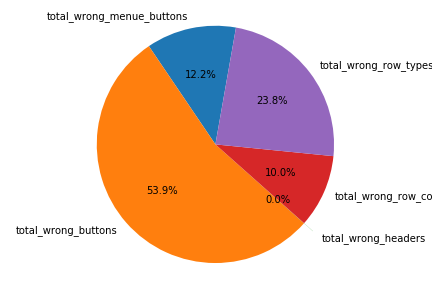
\includegraphics[width=1\linewidth]{predictions_bin12_excluded_p80_error_types_pie_chart}
  \captionof{figure}{Ohne p80}
  \label{fig:fehler_beste80_bin12}
\end{minipage}
\begin{minipage}{.5\textwidth}
  \centering
   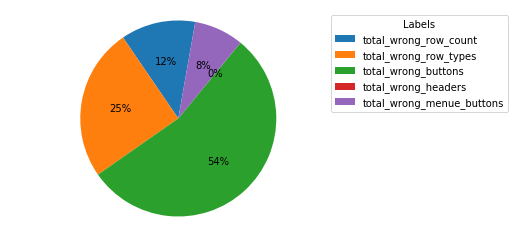
\includegraphics[width=1\linewidth]{predictions_bin12_p80_error_types_pie_chart}
  \captionof{figure}{Nur p80}
  \label{fig:fehler_schlechteste20_bin12}
\end{minipage}%
\end{figure}

Der Unterschied in der Verteilung der Fehlertypen zwischen den ersten 4 Quintilen und dem letzten Quintil ist hier viel geringer, als in dem siebten Experiment. Diesem Modell ist es nicht gelungen, gute Ergebnisse aus den Trainingsdaten zu generieren. Dies unterstreicht die Verteilung der generierten Row-Types in Abbildung~\ref{fig:bin12_row_type}. Hier ist zusehen, dass das Modell es nicht lernen konnten die verschiedenen Typen sicher zu unterscheiden. Ein Großteil wird als Typ 4 erkannt, ca. 60\%, und der Rest ist nicht regelmäßig verteilt.

\begin{figure}[h]
\centering
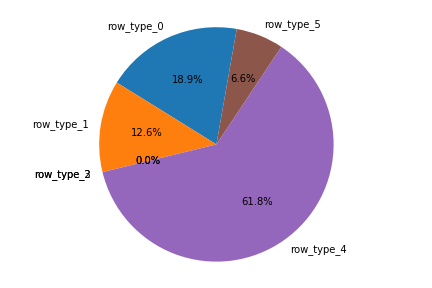
\includegraphics[width=0.5\textwidth]{predictions_bin12_predicted_row_type_distribution}
\caption{Verteilung Row Types}
\label{fig:bin12_row_type}
\end{figure}

\subsubsection*{Fazit}





\subsection{10. Trainingsversuch}

\begin{comment}
%Language: LSTM 256 units
%Decoder 512 units

python train.py ../../data/rfp_data_no_body_3096_11.10.
2018/ ../bin13/ 1

4010/4009 [==============================] - 1737s 433ms/step - loss: 0.7700
Epoch 2/10
4010/4009 [==============================] - 1730s 431ms/step - loss: 0.2034
Epoch 3/10
4010/4009 [==============================] - 1755s 438ms/step - loss: 0.1963
Epoch 4/10
4010/4009 [==============================] - 1742s 434ms/step - loss: 0.1945
Epoch 5/10
4010/4009 [==============================] - 1725s 430ms/step - loss: 0.1929
Epoch 6/10
4010/4009 [==============================] - 1726s 430ms/step - loss: 0.1923
Epoch 7/10
4010/4009 [==============================] - 1725s 430ms/step - loss: 0.1931
Epoch 8/10
4010/4009 [==============================] - 1724s 430ms/step - loss: 0.1923
Epoch 9/10
4010/4009 [==============================] - 1725s 430ms/step - loss: 0.1924
Epoch 10/10
4010/4009 [==============================] - 1725s 430ms/step - loss: 0.1920
\end{comment}



\subsubsection*{Einführung}

Mit diesem Versuch, wird getestet, ob eine reine LSTM-Lösung mit mehr Parametern funktionieren könnte. 

\subsubsection*{Datenset}

Hier wurde das Datenset aus dem sechsten Trainingsversuch verwendet.

\subsubsection*{Veränderte Parameter}

Um zu überprüfen, ob es reicht das Sprach-Modell komplexer zu gestalten, wurde die Anzahl der LSTM Units dieses Teils verdoppelt. 

\begin{verbatim}

Layer (type)                    Output Shape         Param #     Connected to
==============================================================================
input_1 (InputLayer)            (None, 256, 256, 3)  0
______________________________________________________________________________
input_2 (InputLayer)            (None, 48, 23)       0
______________________________________________________________________________
sequential_1 (Sequential)       (None, 48, 1024)     104098080   input_1[0][0]
______________________________________________________________________________
sequential_2 (Sequential)       (None, 48, 256)      812032      input_2[0][0]
______________________________________________________________________________
concatenate_1 (Concatenate)     (None, 48, 1280)     0           sequential_1[1][0]
                                                                 sequential_2[1][0]
______________________________________________________________________________
lstm_3 (LSTM)                   (None, 48, 512)      3672064     concatenate_1[0][0]
______________________________________________________________________________
lstm_4 (LSTM)                   (None, 512)          2099200     lstm_3[0][0]
______________________________________________________________________________
dense_3 (Dense)                 (None, 23)           11799       lstm_4[0][0]
==============================================================================

Total params: 110,693,175
\end{verbatim}

In der Ebene \texttt{sequential\_2}, kommen 256 anstatt 128 Units vor.

\subsubsection*{Ergebnis}

Das Training konvergierte, erzeugt ein sehr schlechtes Ergebnis. Es konnten zwar alle 619 Testdaten kompiliert werden, die Scorings sind nicht Konkurrenzfähig zu den siebten Versuch - aber besser als die Ergebnisse des Neuntens.

Die Analyse der Fehlerverteilung ergibt folgende Lageparameter in Abbildung~\ref{fig:lage_bin13}. Die Verteilung der Fehler-Scores ist in Abbildung~\ref{fig:hist_bin13} gegeben.

\begin{figure}
\centering
\begin{minipage}{.5\textwidth}
  \centering
  \begin{description}
	\item[Arithmetisches Mittel] $23.81$	
	\item[Geometrisches Mittel] $22.98$
	\item[Harmonisches Mittel] $22.14$
	\item[Quintile] p20: $19$, p40: $22$, p60: $24$, p80: $31$
	\item[Median] $23$
	\item[Modus] $22$
	\item[Vorkommen Modus] $57$
	\item[Gesamt Fehler Score] 14739
	\item[Anzahl Token Testset] 36751 
	\item[Anzahl generierter Token] 34664
	\item[Score pro Token Testset]  0.40
\end{description}
  \captionof{figure}{Lageparameter}
  \label{fig:lage_bin13}
\end{minipage}%
\begin{minipage}{.5\textwidth}
  \centering
  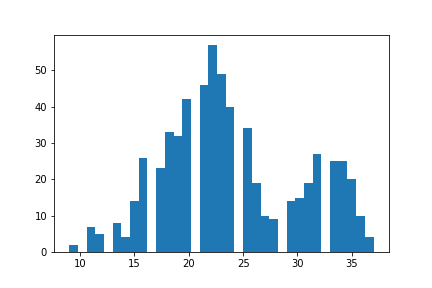
\includegraphics[width=1\linewidth]{predictions_bin13_histogramm}
  \captionof{figure}{Fehlerverteilung}
  \label{fig:hist_bin13}
\end{minipage}
\end{figure}

Auffallend ist hier, dass die Verteilung der Fehler Scores viel gleichmäßiger als in den Versuchen Sieben und Neun ist. Die Abstände der verschiedenen Mittel sowie die der Quintile sind geringer. Im Vergleich zum neunten Versuch ist der Median Score um 10 geringer. 

\begin{figure}
\centering
\begin{minipage}{.5\textwidth}
  \centering
  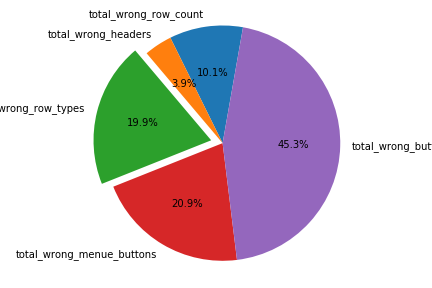
\includegraphics[width=1\linewidth]{predictions_bin13_total_error_types_pie_chart}
  \captionof{figure}{Gesamt}
  \label{fig:fehler_gesamt_bin13}
\end{minipage}%
\begin{minipage}{.5\textwidth}
  \centering
  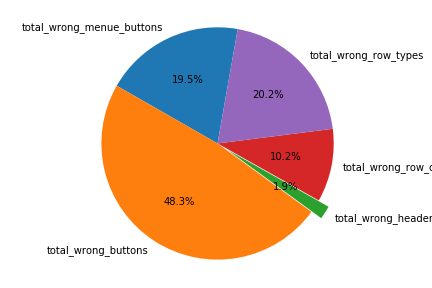
\includegraphics[width=1\linewidth]{predictions_bin13_excluded_p80_error_types_pie_chart}
  \captionof{figure}{Ohne p80}
  \label{fig:fehler_beste80_bin13}
\end{minipage}
\begin{minipage}{.5\textwidth}
  \centering
   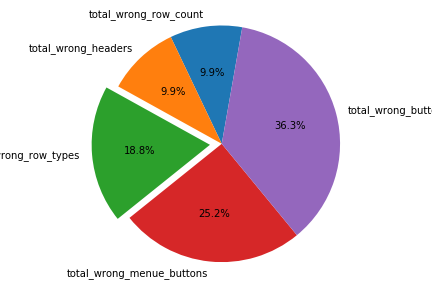
\includegraphics[width=1\linewidth]{predictions_bin13_p80_error_types_pie_chart}
  \captionof{figure}{Nur p80}
  \label{fig:fehler_schlechteste20_bin13}
\end{minipage}%
\end{figure}

Auffallend ist jedoch in Abbildung~\ref{fig:fehler_gesamt_bin13}, dass dieses Modell den bisher höchsten Anteil an falsch zugeordneten \texttt{header}-Elementen hat. Die bisherigen konvergierten Modelle konnten diese jeweils perfekt zuordnen. 

Schließlich kommt der letzte Punkt der Analyse, die Verteilung der generierten Row Typen. Hier schneidet dieses Modell am aller schlechtesten ab. Es generiert in für Datei aus dem Testset immer nur einen von zwei Row Types. 

\begin{figure}[h]
\label{fig:bin13_row_type}

\centering
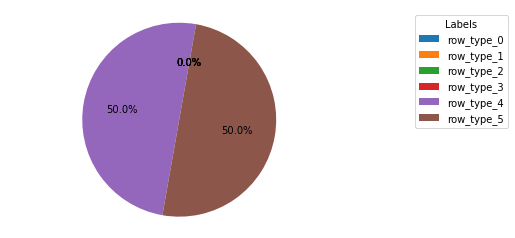
\includegraphics[width=0.5\textwidth]{predictions_bin13_predicted_row_type_distribution}
\caption{Verteilung Row Types}
\end{figure}


\subsubsection*{Fazit}

Obwohl dieses Modell mit großer LSTM Architektur knappe 2.5 Millionen Parameter mehr hat, sind die Ergebnisse viel schlechter. Besonders die drei fehlenden Row-Types fallen hier ins Gewicht. Zunächst wurde angenommen, dass dieses Modell gleich gut oder besser wie die reine GRU Architektur aus Versuch Sieben sein könnte. Die LSTMs performen bisher schlechter für diesen Task. 




\subsection{11. Trainingsversuch}\label{sec:elf}
%Language: GRU 192 units
%Decoder GRU 768 units

%bin14

\subsubsection*{Einführung}
In diesem Versuch soll heraus gefunden werden, ob eine größere GRU-Architektur ein noch besseres Ergebniss liefern könnte.

\subsubsection*{Datenset}

Hier wurde das Datenset aus dem sechsten Trainingsversuch verwendet.


\subsubsection*{Veränderte Parameter}

Es wurden sowohl die Sprach-Ebene, als auch die Decoder-Ebene vergrößert.

\begin{verbatim}
Layer (type)                    Output Shape         Param #     Connected to
=============================================================================
input_1 (InputLayer)            (None, 256, 256, 3)  0
_____________________________________________________________________________
input_2 (InputLayer)            (None, 48, 23)       0
_____________________________________________________________________________
sequential_1 (Sequential)       (None, 48, 1024)     104098080   input_1[0][0]
_____________________________________________________________________________
sequential_2 (Sequential)       (None, 48, 192)      346176      input_2[0][0]
_____________________________________________________________________________
concatenate_1 (Concatenate)     (None, 48, 1216)     0           sequential_1[1][0]
                                                                 sequential_2[1][0]
_____________________________________________________________________________
gru_3 (GRU)                     (None, 48, 768)      4573440     concatenate_1[0][0]
_____________________________________________________________________________
gru_4 (GRU)                     (None, 768)          3541248     gru_3[0][0]
_____________________________________________________________________________
dense_3 (Dense)                 (None, 23)           17687       gru_4[0][0]
=============================================================================

Total params: 112,576,631

\end{verbatim}

Hier kann man sehen, dass in der Ebene \texttt{sequential\_2} in der Ebene \texttt{gru\_3} die Unit-Anzahl vergrößert wurde. Von 128 auf 192, bzw. von 512 auf 786.

\subsubsection*{Ergebnis}

Auch dieses Netz konvergiert, leider ist das Ergebnis gegenüber Versuch Sieben nicht besser geworden.

\begin{figure}
\centering
\begin{minipage}{.5\textwidth}
  \centering
  \begin{description}
	\item[Arithmetisches Mittel] $20.10$	
	\item[Geometrisches Mittel] $19.23$
	\item[Harmonisches Mittel] $18.38$
	\item[Quintile] p20: $16$, p40: $19$, p60: $21$, p80: $22$
	\item[Median] $20$
	\item[Modus] $21$
	\item[Vorkommen Modus] $85$
	\item[Gesamt Fehler Score] 12442
	\item[Anzahl Token Testset] 36751 
	\item[Anzahl generierter Token] 33680
	\item[Score pro Token Testset]  0.34
\end{description}
  \captionof{figure}{Lageparameter}
  \label{fig:lage_bin14}
\end{minipage}%
\begin{minipage}{.5\textwidth}
  \centering
  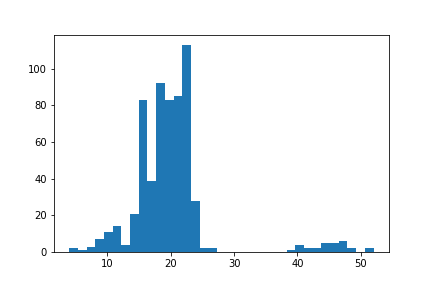
\includegraphics[width=1\linewidth]{predictions_bin14_histogramm}
  \captionof{figure}{Fehlerverteilung}
  \label{fig:hist_bin14}
\end{minipage}
\end{figure}

Der Hauptteil der Fehler-Scores liegt um die Zwanzig, mit ein paar wenigen im niedrigeren oder höheren Bereich. Zu sehen ist das sehr gut in der Abbildung~\ref{fig:hist_bin14}. 

\begin{figure}
\centering
\begin{minipage}{.5\textwidth}
  \centering
  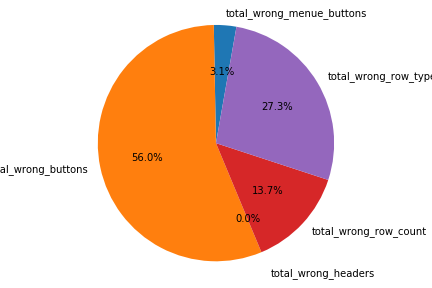
\includegraphics[width=1\linewidth]{predictions_bin14_total_error_types_pie_chart}
  \captionof{figure}{Gesamt}
  \label{fig:fehler_gesamt_bin14}
\end{minipage}%
\begin{minipage}{.5\textwidth}
  \centering
  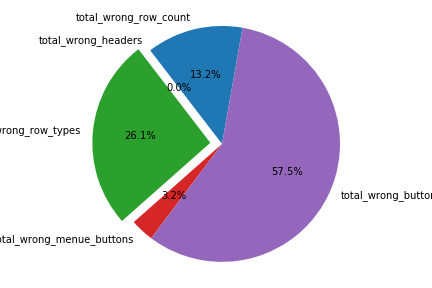
\includegraphics[width=1\linewidth]{predictions_bin14_excluded_p80_error_types_pie_chart}
  \captionof{figure}{Ohne p80}
  \label{fig:fehler_beste80_bin14}
\end{minipage}
\begin{minipage}{.5\textwidth}
  \centering
   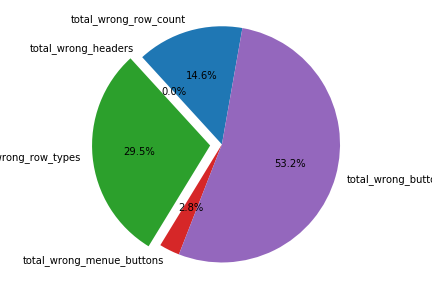
\includegraphics[width=1\linewidth]{predictions_bin14_p80_error_types_pie_chart}
  \captionof{figure}{Nur p80}
  \label{fig:fehler_schlechteste20_bin14}
\end{minipage}
\end{figure}

In Abbildungen ~\ref{fig:fehler_gesamt_bin14}-~\ref{fig:fehler_schlechteste20_bin14} ist zu sehen, dass die Verteilung der Fehler-Type nach Fehler Anzahl relativ gleichmäßig liegt. Die Daten, welche die Meisten Fehler erzeugt haben, erzeugen die gleichen Arten wie der Gesamtmenge. Daher liegt die Fehlerursache nicht in besonders komplexen Screenshots, sondern bei einer schlechten Klassifizierung.

Schlussendlich ist zu sehen, wie schlecht das Modell bei der richtigen Einordnung von den Row-Types anschneidet in Abbildung~\ref{fig:bin14_row_type}. Es kann nicht zwischen den einzelnen Typen unterscheiden.


\begin{figure}[h]
\centering
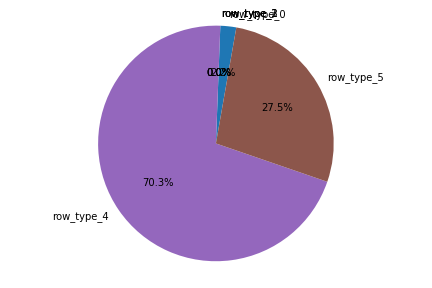
\includegraphics[width=0.5\textwidth]{predictions_bin14_predicted_row_type_distribution}
\caption{Verteilung Row Types}
\label{fig:bin14_row_type}
\end{figure}


\subsubsection*{Fazit}

Wieso performt dieses Modell, obwohl es doch größer ist so viel schlechter als Versuch Sieben? Hier hat man es mit einem klassischen Fall des Overfittings zu tun. Das Modell war hier so komplex, dass es die Beschreibungen aller Trainingsdaten auswendig lernen konnte. Dadurch sah das Training gut aus, das Testen hingegen zeigt, dass es nicht gut verallgemeinern konnte.


\subsection{12. Trainingsversuch}
%Language: GRU 128 units
%Decoder GRU 512 units
%CONTEXT_64
%bin15
\subsubsection*{Einführung}

In diesem Versuch wird überprüft, ob eine Vergrößerung der \texttt{CONTEXT\_LENGTH} das Ergebnis positiv beeinflusst, und wenn ja wie stark. 

\subsubsection*{Datenset}

Hier wurde das Datenset aus dem sechsten Trainingsversuch verwendet.

\subsubsection*{Veränderte Parameter}

Die \texttt{CONTEXT\_LENGTH} wurde von 48 auf 64 (Anmerkung: die Median Token-Sequenz-Länge des Trainingssets ist 62) erhöht. Die wirkt sich folgendermaßen auf die Architektur aus:
\begin{verbatim}

_____________________________________________________________________________
Layer (type)                    Output Shape         Param #     Connected to
=============================================================================
input_1 (InputLayer)            (None, 256, 256, 3)  0
_____________________________________________________________________________
input_2 (InputLayer)            (None, 64, 23)       0
_____________________________________________________________________________
sequential_1 (Sequential)       (None, 64, 1024)     104098080   input_1[0][0]
_____________________________________________________________________________
sequential_2 (Sequential)       (None, 64, 128)      157056      input_2[0][0]
_____________________________________________________________________________
concatenate_1 (Concatenate)     (None, 64, 1152)     0           sequential_1[1][0]
                                                                 sequential_2[1][0]
_____________________________________________________________________________
gru_3 (GRU)                     (None, 64, 512)      2557440     concatenate_1[0][0]
_____________________________________________________________________________
gru_4 (GRU)                     (None, 512)          1574400     gru_3[0][0]
_____________________________________________________________________________
dense_3 (Dense)                 (None, 23)           11799       gru_4[0][0]
=============================================================================

Trainable params: 108,398,775

\end{verbatim}

Der \texttt{Output Shape} der Ebenen \texttt{input\_2},  \texttt{sequential\_1},  \texttt{sequential\_2},  \texttt{concatenate\_1} und \texttt{gru\_3} spiegelt jeweils in der ersten Dimension die nun erhöhte \texttt{CONTEXT\_LENGTH} wieder.
Ansonsten ist das Modell gleich wie das des siebten Versuchs.
\subsubsection*{Ergebnis}

\begin{figure}
\centering
\begin{minipage}{.5\textwidth}
  \centering
  \begin{description}
	\item[Arithmetisches Mittel] $6.44$	
	\item[Geometrisches Mittel] $5.78$
	\item[Harmonisches Mittel] $5.07$
	\item[Quintile] p20: $4$, p40: $6$, p60: $7$, p80: $8$
	\item[Median] $6$
	\item[Modus] $6$
	\item[Vorkommen Modus] $116$
	\item[Gesamt Fehler Score] 3989
	\item[Anzahl Token Testset] 36751 
	\item[Anzahl generierter Token] 36869
	\item[Score pro Token Testset]  0.1085
\end{description}
  \captionof{figure}{Lageparameter}
  \label{fig:lage_bin15}
\end{minipage}%
\begin{minipage}{.5\textwidth}
  \centering
  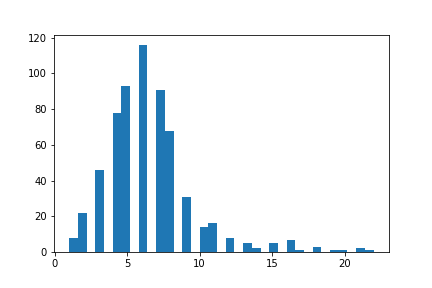
\includegraphics[width=1\linewidth]{predictions_bin15_histogramm}
  \captionof{figure}{Fehlerverteilung}
  \label{fig:hist_bin15}
\end{minipage}
\end{figure}

Im Vergleich zu das Modell vom Versuch Sieben, performt dieses Modell besser, siehe \ref{fig:lage_bin10}. Der Fehler-Score ist etwas geringer, aber im Modell von Versuch Sieben ist das zweite Quintil, sowie der Modus jeweils um eine Einheit niedriger. 

\begin{figure}
\centering
\begin{minipage}{.5\textwidth}
  \centering
  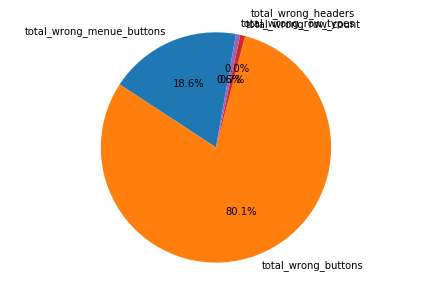
\includegraphics[width=1\linewidth]{predictions_bin15_total_error_types_pie_chart}
  \captionof{figure}{Gesamt}
  \label{fig:fehler_gesamt_bin15}
\end{minipage}%
\begin{minipage}{.5\textwidth}
  \centering
  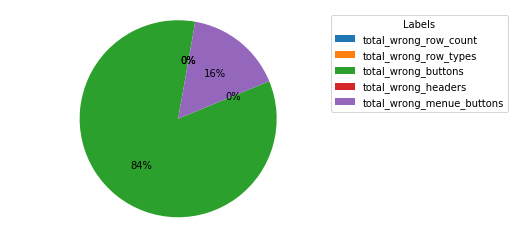
\includegraphics[width=1\linewidth]{predictions_bin15_excluded_p80_error_types_pie_chart}
  \captionof{figure}{Ohne p80}
  \label{fig:fehler_beste80_bin15}
\end{minipage}
\begin{minipage}{.5\textwidth}
  \centering
   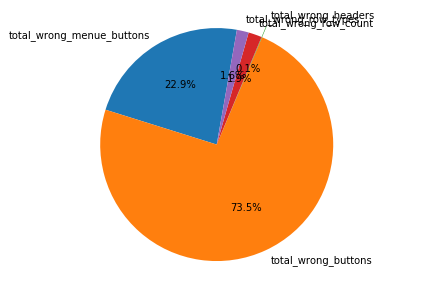
\includegraphics[width=1\linewidth]{predictions_bin15_p80_error_types_pie_chart}
  \captionof{figure}{Nur p80}
  \label{fig:fehler_schlechteste20_bin15}
\end{minipage}
\end{figure}

Die Verteilung der Fehler im letzten Quintil ist ebenso sehr gut; es gab nur 22 mal das Auftreten von falschen Row-Klassifizierungen. Zum Vergleich, im siebten Versuch gab es 174 falsche Klassifizierungen des Row-Types.

\begin{figure}[h]
\centering
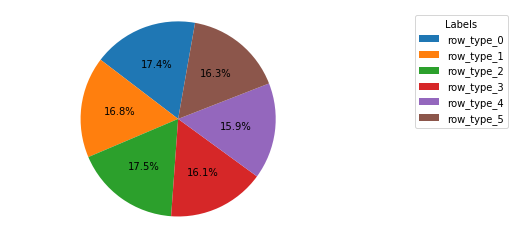
\includegraphics[width=0.5\textwidth]{predictions_bin15_predicted_row_type_distribution}
\caption{Verteilung Row Types}
\label{fig:bin15_row_type}
\end{figure}

Daher ist auch die Verteilung der Row Type sehr gleichmäßig, zu sehen in Abbildung~\ref{fig:bin15_row_type}. 
Der Fehler Score ist gegenüber Versuch Sieben um ca. 18\% gesunken. 
Interessant ist, dass dieses Modell 276\% der Fehler des siebten Versuchs in den Menü-Buttons macht. Außerdem hat es einmal einen falschen Header identifiziert. Bei der Anzahl der falschen Buttons gibt es kaum einen Unterschied zum siebten Modell.

\subsubsection*{Fazit}
Aufgrund der längeren \texttt{CONTEXT\_LENGTH} ist das Ergebnis sehr viel besser geworden. Row-Types werden hier mit am zuverlässigsten erkannt, was wahrscheinlich an der verlängerten \texttt{CONTEXT\_LENGTH} liegt, da das Modell so auf jeden Fall die aktuelle Row als auch die davor gleichzeitig im Speicher haben kann. Leider gibt es Abspriche in der Qualität der Menüs, da hat fast 3 mal so viele Fehler gemacht wie der Vergleich. Die ist aber zu verschmerzen, da Performance der Rows so außerordentlich gut ist. Vielleicht ist das Modell ein bisschen zu einfach um die Komplexität der DSL und der Screenshots ausreichend abzubilden. 

\subsection{13. Trainingsversuch}
%Language: GRU 92 units
%Decoder GRU 386 units

%bin16

\subsubsection*{Einführung}

Hier wird eine vereinfachte Variante des siebten Modells genutzt, um zu testen, ob es so besser verallgemeinert.

\subsubsection*{Datenset}

Hier wurde das Datenset aus dem sechsten Trainingsversuch verwendet.

\subsubsection*{Veränderte Parameter}

Sowohl der Sprach- als auch der Decoder-Teil des Modells wurden verkleinert. Die Anzahl der rekurrenten \texttt{Units} sind von 128 auf 92 im Sprach-Teil und von 512 auf 386 im Decoder-Teil reduziert worden.

\begin{verbatim}
Layer (type)                    Output Shape         Param #     Connected to
=============================================================================
input_1 (InputLayer)            (None, 256, 256, 3)  0
_____________________________________________________________________________
input_2 (InputLayer)            (None, 48, 23)       0
_____________________________________________________________________________
sequential_1 (Sequential)       (None, 48, 1024)     104098080   input_1[0][0]
_____________________________________________________________________________
sequential_2 (Sequential)       (None, 48, 92)       83076       input_2[0][0]
_____________________________________________________________________________
concatenate_1 (Concatenate)     (None, 48, 1116)     0           sequential_1[1][0]
                                                                 sequential_2[1][0]
_____________________________________________________________________________
gru_3 (GRU)                     (None, 48, 386)      1740474     concatenate_1[0][0]
_____________________________________________________________________________
gru_4 (GRU)                     (None, 386)          895134      gru_3[0][0]
_____________________________________________________________________________
dense_3 (Dense)                 (None, 23)           8901        gru_4[0][0]


Trainable params: 106,825,665
\end{verbatim}

Diese Änderung sieht man in den Ebenen \texttt{sequential\_2} sowie \texttt{gru\_2} und \texttt{gru\_4}.
Durch die Verkleinerung der RNNs, ist das Modell um knapp zwei Millionen Parameter kleiner geworden.

\subsubsection*{Ergebnis}


Wie in Abbildung~\ref{fig:lage_bin16} zu sehen ist, sind alle Lageparameter schlechter als die bisherigen guten Ergebnisse.

\begin{figure}
\centering
\begin{minipage}{.5\textwidth}
  \centering
  \begin{description}
	\item[Arithmetisches Mittel] $16.71$	
	\item[Geometrisches Mittel] $15.25$
	\item[Harmonisches Mittel] $13.62$
	\item[Quintile] p20: $11$, p40: $15$, p60: $17$, p80: $22$
	\item[Median] $16$
	\item[Modus] $16$
	\item[Vorkommen Modus] $54$
	\item[Gesamt Fehler Score] 10342
	\item[Anzahl Token Testset] 36751 
	\item[Anzahl generierter Token] 36047
	\item[Score pro Token Testset]  0.28
\end{description}
  \captionof{figure}{Lageparameter}
  \label{fig:lage_bin16}
\end{minipage}%
\begin{minipage}{.5\textwidth}
  \centering
  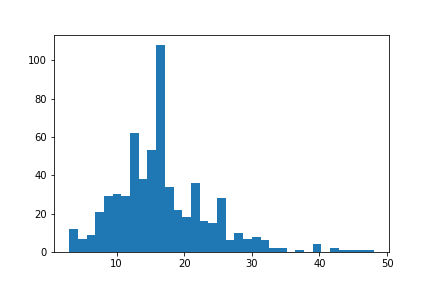
\includegraphics[width=1\linewidth]{predictions_bin16_histogramm}
  \captionof{figure}{Fehlerverteilung}
  \label{fig:hist_bin16}
\end{minipage}
\end{figure}

Im Vergleich der Lageparameter zu dem zehnten Trainingsversuch (LSTM mit mehr Parametern), gibt es hier einen geringeren Fehler-Score. Es ist jedoch zu sehen, an den Abbildungen~\ref{fig:fehler_gesamt_bin16} bis ~\ref{fig:fehler_schlechteste20_bin16}, dass dieFehlerverteilung überall gleich ist, egal in welchem Quintil.

\begin{figure}
\centering
\begin{minipage}{.5\textwidth}
  \centering
  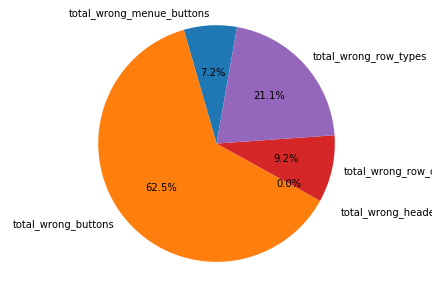
\includegraphics[width=1\linewidth]{predictions_bin16_total_error_types_pie_chart}
  \captionof{figure}{Gesamt}
  \label{fig:fehler_gesamt_bin16}
\end{minipage}%
\begin{minipage}{.5\textwidth}
  \centering
  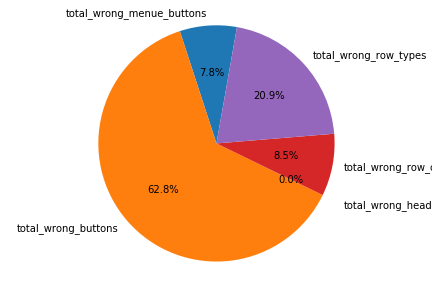
\includegraphics[width=1\linewidth]{predictions_bin16_excluded_p80_error_types_pie_chart}
  \captionof{figure}{Ohne p80}
  \label{fig:fehler_beste80_bin16}
\end{minipage}
\begin{minipage}{.5\textwidth}
  \centering
   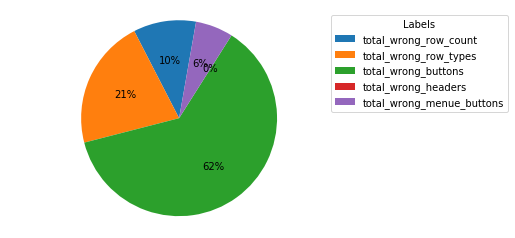
\includegraphics[width=1\linewidth]{predictions_bin16_p80_error_types_pie_chart}
  \captionof{figure}{Nur p80}
  \label{fig:fehler_schlechteste20_bin16}
\end{minipage}
\end{figure}

An der Verteilung der generierten Row Types in Abbildung~\ref{fig:bin16_row_type} erkennt man, dass diese Modell es nicht gelernt hat die Typen zuverlässig zu unterscheiden.

\begin{figure}[h]
\centering
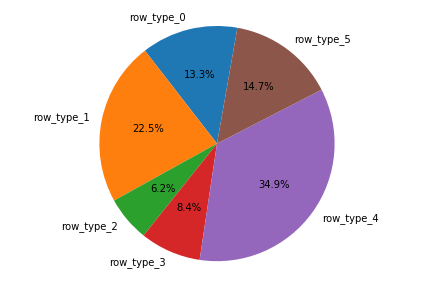
\includegraphics[width=0.5\textwidth]{predictions_bin16_predicted_row_type_distribution}
\caption{Verteilung Row Types}
\label{fig:bin16_row_type}
\end{figure}

\subsubsection*{Fazit}
Durch das Reduzieren der \texttt{Units} der RNNs ist das Modell schlicht zu simpel geworden. Obwohl es die richtige Grammatik lernen konnte - es hat keine Token-Sequenzen erzeugt, die nicht kompiliert werden konnte.

\subsection{14. Trainingsversuch}

\subsubsection*{Einführung}

Der Ansatz aus dem 12. Versuch, die vergrößerte \texttt{CONTEXT\_LENGTH} wurde hier verwendet, in Kombination mit einem etwas größeren Netzwerk. In den bisherigen Versuchen gab es stets viele falsch farbige Buttons, vielleicht kann dieses Problem mit einer leicht vergrößerten Decoder Architektur behoben werden.

\subsubsection*{Datenset}

Hier wurde das Datenset auf dem sechsten Trainingsversuch verwendet.

\subsubsection*{Veränderte Parameter}

Die Anzahl der GRUs in dem Decoder-Teil des Netzwerkes wurde von 512 auf 564 erhöht. Außerdem wurden 20 Epochen trainiert statt nur 10.

\subsubsection*{Ergebnis}

Diese Model performt sogar noch besser als das Modell des Siebten und Zwölften Versuches.

\begin{figure}
\centering
\begin{minipage}{.5\textwidth}
  \centering
  \begin{description}
	\item[Arithmetisches Mittel] $5.85$	
	\item[Geometrisches Mittel] $5.06$
	\item[Harmonisches Mittel] $4.43$
	\item[Quintile] p20: $3$, p40: $5$, p60: $6$, p80: $7$
	\item[Median] $5$
	\item[Modus] $6$
	\item[Vorkommen Modus] $116$
	\item[Gesamt Fehler Score] 3621
	\item[Anzahl Token Testset] 36751 
	\item[Anzahl generierter Token] 36879
	\item[Score pro Token Testset]  0.0985
\end{description}
  \captionof{figure}{Lageparameter}
  \label{fig:lage_bin16}
\end{minipage}%
\begin{minipage}{.5\textwidth}
  \centering
  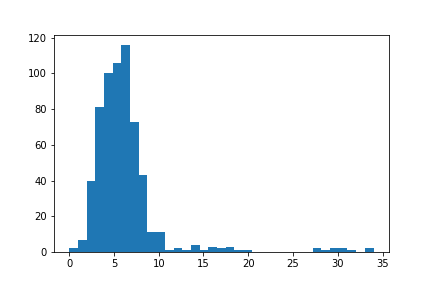
\includegraphics[width=1\linewidth]{predictions_bin18_2_histogramm}
  \captionof{figure}{Fehlerverteilung}
  \label{fig:hist_bin18}
\end{minipage}
\end{figure}

Im Vergleich zum Versuch Zwölf, macht dieses Modell sehr viel weniger Fehler bei Bestimmung der richten Anzahl der Menü Buttons (223 gegenüber 780) aber bei Bestimmung der richtigen Buttons im Content ist Performance ein wenig schlechter (2963 gegenüber 2751). Das aktuelle Modell bestimmt mehr falsche Row Types, 32 gegenüber 13 in Versuch Zwölf, aber dafür generiert es weniger oft die falsche Row Anzahl (33 gegenüber 45). 

\begin{figure}
\centering
\begin{minipage}{.33\textwidth}
  \centering
  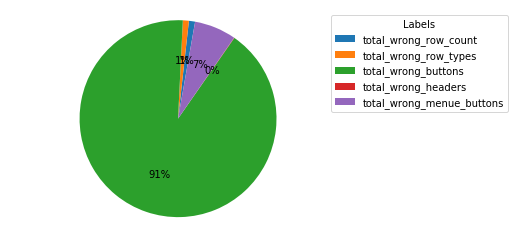
\includegraphics[width=1\linewidth]{predictions_bin18_2_total_error_types_pie_chart}
  \captionof{figure}{Gesamt}
  \label{fig:fehler_gesamt_bin18_2}
\end{minipage}%
\begin{minipage}{.33\textwidth}
  \centering
  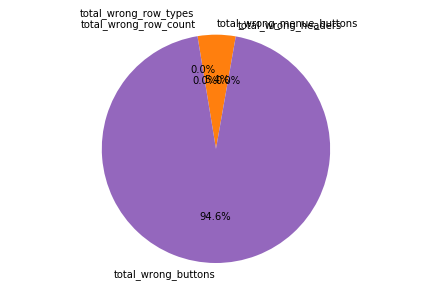
\includegraphics[width=1\linewidth]{predictions_bin18_2_excluded_p80_error_types_pie_chart}
  \captionof{figure}{Ohne p80}
  \label{fig:fehler_beste80_bin18_2}
\end{minipage}
\begin{minipage}{.33\textwidth}
  \centering
   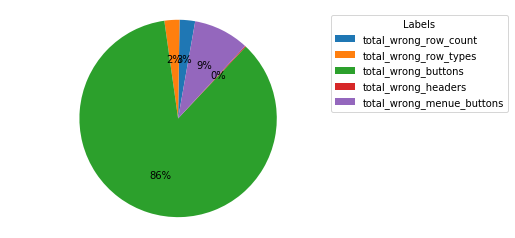
\includegraphics[width=1\linewidth]{predictions_bin18_2_p80_error_types_pie_chart}
  \captionof{figure}{Nur p80}
  \label{fig:fehler_schlechteste20_bin18_2}
\end{minipage}
\end{figure}

\subsubsection*{Fazit}

Der Fehler Score ist etwas geringer als im Versuch 12, aber im Grunde ist die Performance der beiden Modelle ziemlich ähnlich. Die geringe Vergrößerung des Decoder-Teils, hat so nicht zu einer signifikanten Verbesserung beigetragen. Da das Netzwerk bei einer stärkeren Vergrößerung zum Overfitting neigt (vergleiche mit Versuch 11, Abschnitt~\ref{sec:elf}, ist diese Konfiguration des Netzwerkes die Effektivste.

\section{Zusammenfassung der Versuchsergebnisse}

In Tabelle~\ref{tab:comparison} sind die drei Modelle mit der besten Performance aufgeführt.

\begin{table}[]
\begin{tabular}{cccc}
\textbf{Versuch}                           & \textbf{Sieben} & \textbf{Elf} & \textbf{Zwölf} \\
\textbf{Fehler-Score}                      & 4840            & 12442        & 3989           \\
\textbf{Fehler/Token}                      & 0.1317          & 0.34         & 0.1085         \\
\textbf{Aritmetisches Mittel Fehler-Score} & 7.82            & 20.10        & \textbf{6.44}           \\
\textbf{Anzahl Parameter}                  & 108.398.775     & 112.576.631  & 108,398,775   
\end{tabular}
\captionof{table}{Für jede der Metriken gilt: Je kleiner, desto besser}
\label{tab:comparison}
\end{table}

Viele der Versuche sind nicht gut konvergiert oder hatten die Tendenz die Trainingsdaten auswendig zu lernen. Trotz der vielen Fehlschläge, gelang es eine Architektur zu finden, welche die Ansprüche der DSL und der Komplexität der Screenshots abbilden konnte. 
Das Ersetzen der LSTMs zu GRUs zeigte einen erstaunlichen Performance-Schub, genauso mit einer Erhöhung der Kontext Länge, konnte so die Architektur aus Versuch Sieben noch mal verbessert werden, um schließlich bei der Konfiguration aus Versuch Zwölf anzukommen. 


\section{Fazit}

In vielen Bereichen der Sequenz Modellierung performen LSTMs und GRUs auf einer Ebene ohne einen signifikanten Gewinner auf einer der Seiten. Hier, im Bereich der Sprach-Modellierung in Verbindung mit der Analyse eines Screenshots gibt es aber einen klaren Gewinner: Die \textbf{Gated Recurrent Unit}.

Verschiedene Publikationen \cite{paperGRUComparison}, \cite{lstmSearchSpace}, \cite{colahsBlogLSTM} deuteten stets auf eine ungefähre Ausgewogenheit der Scores der beiden RNN Varianten, aber auch darauf, dass, je nach spezieller Domäne eines Problems, eine Variante besser als die andere sein kann.

Die Annahme, die im Rahmen dieser Arbeit getroffen wird, ist, dass die innere Struktur der GRU, siehe Abbildung~\ref{fig:gru}, besonders gut die Eltern/Kind Beziehungen der verwendeten DSL abbilden kann. Durch die in GRUs verwendete Kopplung der \texttt{forget}- und \texttt{add}-Gates kann diese Beziehung vielleicht besser abgebildet werden als in dem Cell-State des LSTMs. Vielleicht haben Fehler, entweder während des Löschens von Informationen aus dem Cell-State, während des Hinzufügen oder dem Maskieren desselben, bei LSTMs das Halten des Token-States zu kompliziert gemacht und dies hat so zu Fehlern in den Eltern/Kind Beziehungen geführt. Dies sieht man besonders bei Versuch zehn, wo auch eine besonders große LSTM-Architektur ein dürftiges Ergebnis produziert. In Abbildung~\ref{fig:bin13_row_type} erkennt man das wirklich schlechte Modellieren der Rows in diesem Ansatz. In Versuch Sieben und Zwölf auf der anderen Seite, sind diese Rows stets korrekt modelliert, woraus geschlossen werden könnte, dass diese GRUs besser in der Lage sind, Eltern/Kind Beziehungen zu modellieren. Darüber sollten in Zukunft noch ausführlichere Forschungsarbeiten verfasst werden.

\section{Bonus Experiment: Ist das Modell komplex genug um aus einer Skizze eine Website zu erstellen?}

Ein Website aus einen Screenshot eines Designs zu erstellen, ist das eine Problem, aber könnte das selbe Modell auch aus einen groben Skizze vollständiges HTML zu erlernen?

\subsection{1. Trainingsversuch}

\subsubsection*{Einführung}

Zunächst muss ein neues Datenset erstellt werden, mit Skizzen von Websiten anstelle von schön designten. Danach wird eins der Modelle mit guter Erkennungsrate genommen und dieses neu trainiert mit skizzierten Websiten.

\subsubsection*{Datenset}

Hier wurden die Token-Sequenzen aus dem sechsten Trainingsversuch genommen, aber das Styling der Websiten wurde mit anderen CSS-Regeln verändert, damit diese Skizziert aussehen. Im ersten Schritt wurden alle Farben und großflächige Hintergründe durch Weiß ersetzt. Anschließen bekamen alle Elemente eine leicht unregelmäßige Outline. Die Ergebnisse des ersten Schritt sind zu sehen in Abbildung~\ref{fig:skizzen}.

\begin{figure}
\centering
\begin{minipage}{.5\textwidth}
  \centering
  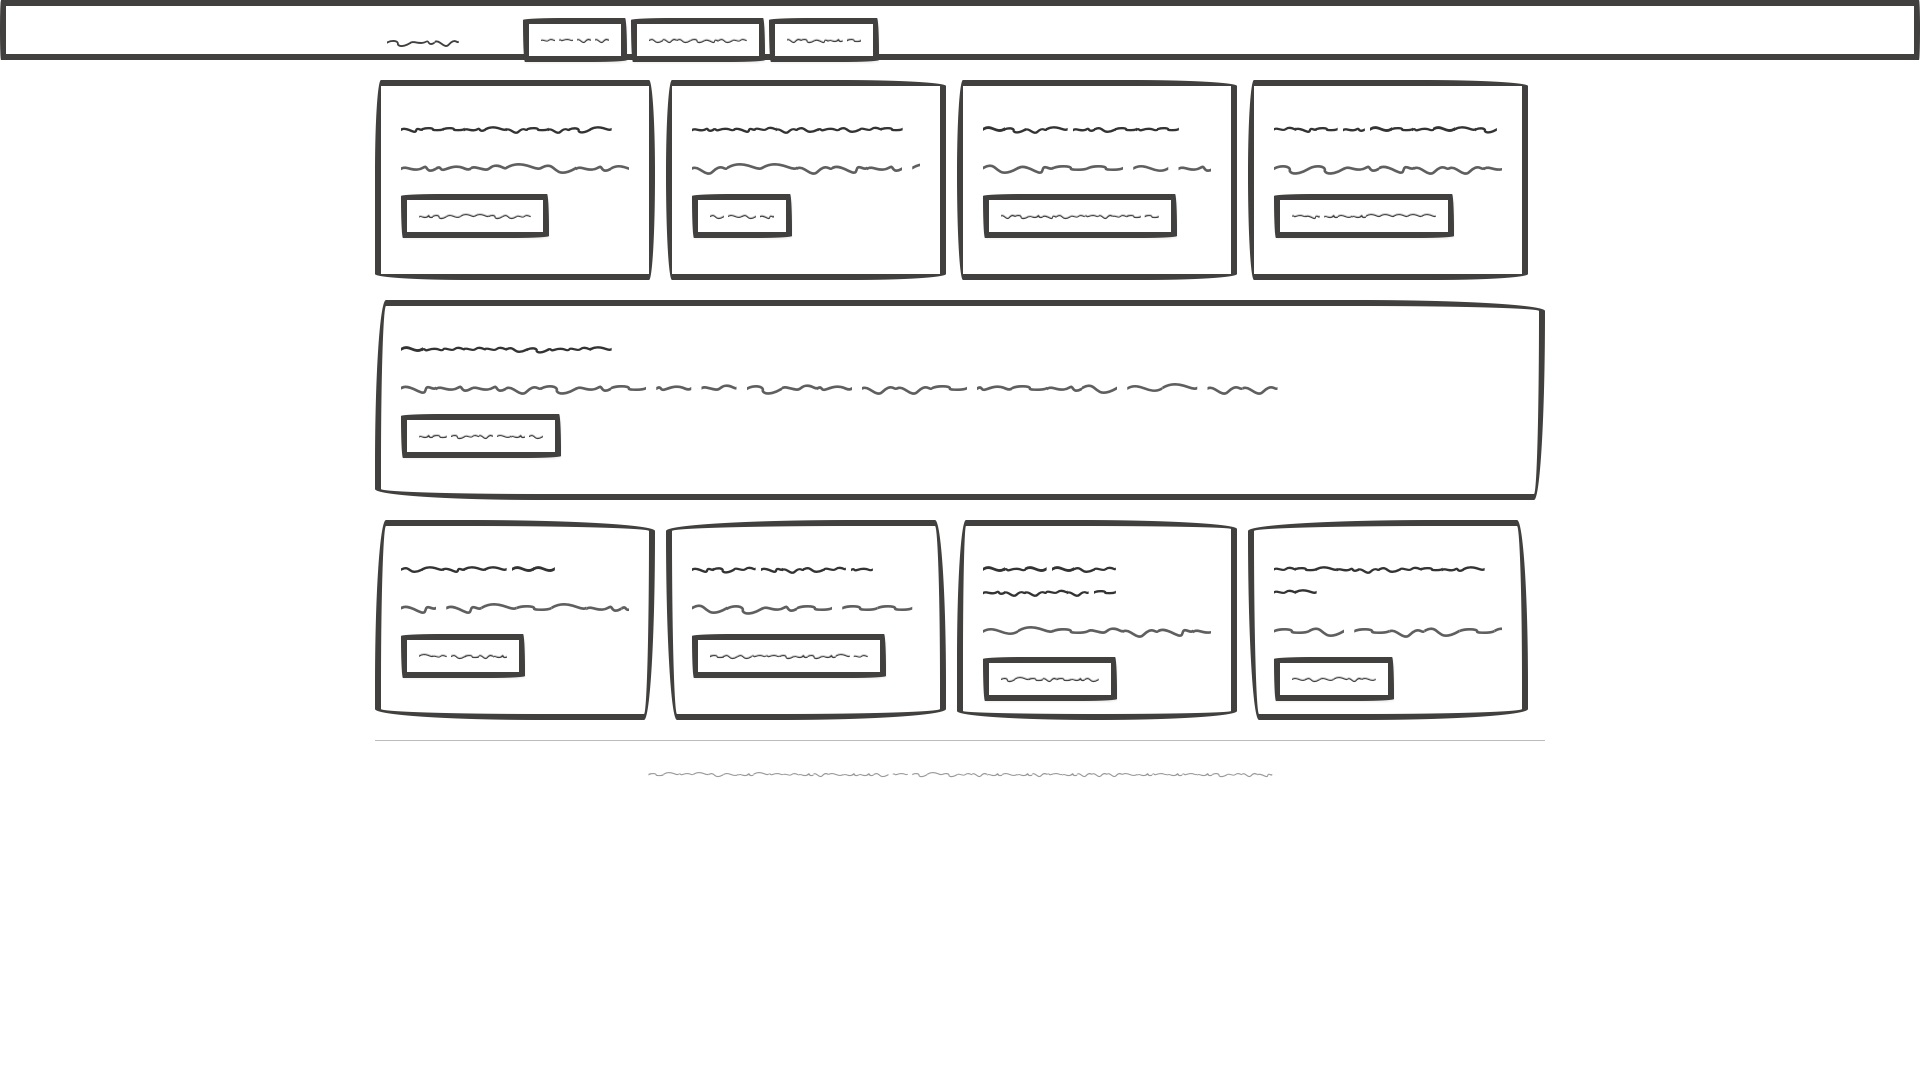
\includegraphics[width=0.8\linewidth]{skizze_1}
\end{minipage}%
\begin{minipage}{.5\textwidth}
  \centering
  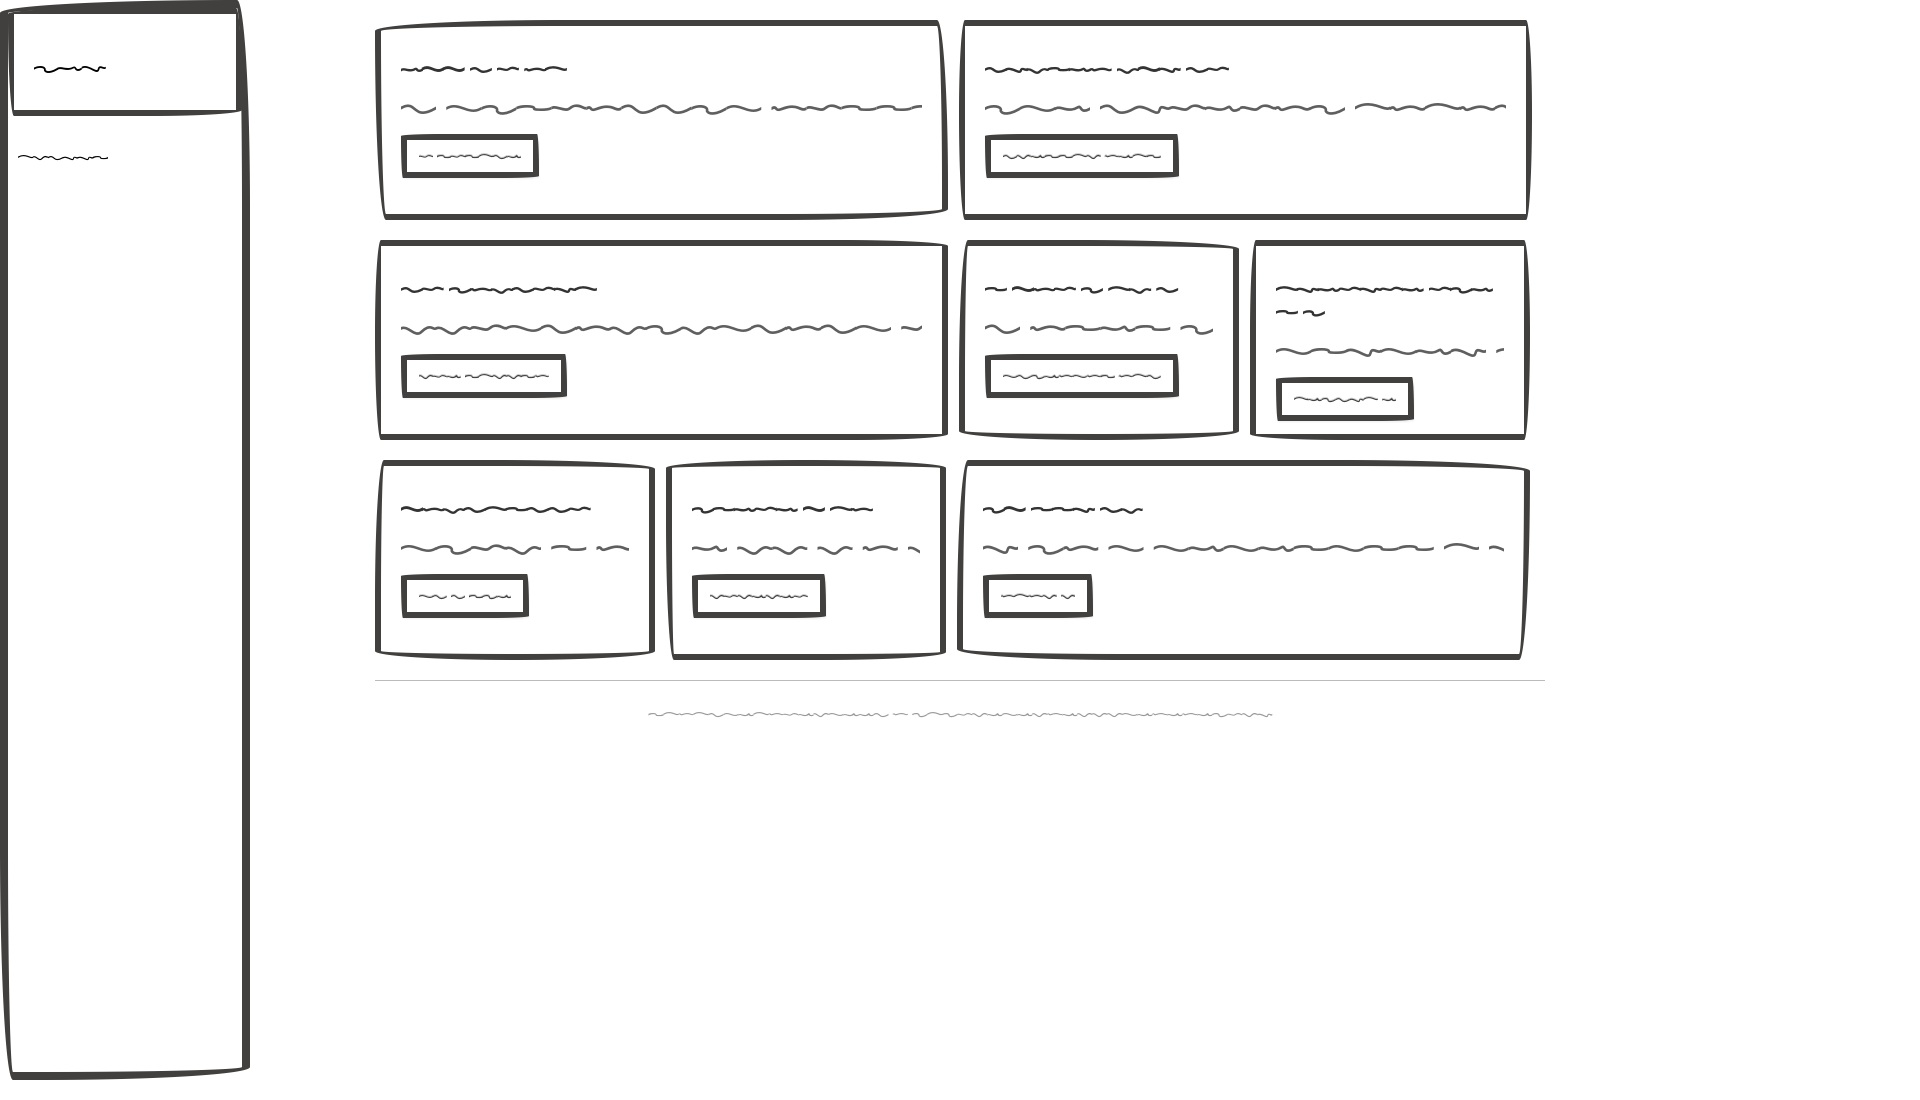
\includegraphics[width=0.8\linewidth]{skizze_2}
\end{minipage}
  \captionof{figure}{Beispiele der Skizzen}
  \label{fig:skizzen}
\end{figure}

Anschließend wurden in einem Zweiten Schritt die Skizzen mit der Python Library \texttt{imagug} noch weiter verzerrt und augmentiert. Für jedes Screenshot wurden 3 unterschiedliche verzerrte Bilder erstellt und auf die Input-Größe des Netzwerkes (256 mal 256 Pixel) skaliert, siehe Abbildung~\ref{fig:skizzen_aug}.

\begin{figure}
\centering
\begin{minipage}{.5\textwidth}
  \centering
  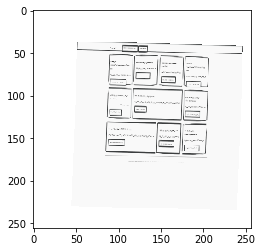
\includegraphics[width=0.8\linewidth]{skizze_aug_1}
\end{minipage}%
\begin{minipage}{.5\textwidth}
  \centering
  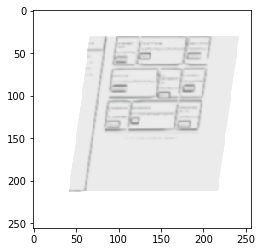
\includegraphics[width=0.8\linewidth]{skizze_aug_2}
\end{minipage}
  \captionof{figure}{Beispiele der augmentierten Trainingsdaten}
  \label{fig:skizzen_aug}
\end{figure}

Während dem Augmentieren wurden folgende Schritte ausgeführt: 
\begin{description}
	\item[Skalierung] In X- und Y-Ausrichtung auf jeweils 70 bis 80\% der original Größe.
	\item[Verschiebung] Verschieben des Bildes um bis zu $\pm$ 10\% auf beiden Achsen.
	\item[Rotation] Um jeweils bis zu $\pm 10^\circ$
	\item[Scherung]  Scherung des Bildes um bis zu $\pm 8^\circ$ auf beiden Achsen.
	\item[Helligkeitsreduktion] Abdunkelung des Bildes bei 50\% aller Bilder um bis zu 15\%
	\item[Weichzeichnung] 50\% der Bilder wurden mit einem Sigma zwischen 0 und 1.2 weichgezeichnet.
\end{description}

All diese Schritte haben zum Ziel, dass das Modell mit Fotos einer Skizze arbeiten kann. Da es viel zu viel Aufwand ist, echte Skizzen als Trainingsdaten zu verwenden, wird getestet ob man diese so nachbilden kann.

\subsubsection*{Veränderte Parameter}

Das Modell des letzten Versuch wurde genutzt.
                 
\subsubsection*{Ergebnis}
   
Leider führte das Training zu keiner Konvergenz des Netzwerkes.
Siehe Abbildung~\ref{fig:loss_drawn_standart}.

\begin{figure}[h]
\centering
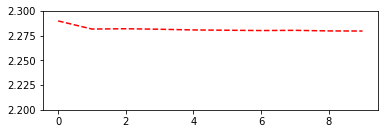
\includegraphics[width=0.5\textwidth]{loss_drawn_standart}
\caption{Loss des 1. Extra-Training}
\label{fig:loss_drawn_standart}
\end{figure}


\subsubsection*{Fazit}

Da das Datenset aus komplexeren Bildern bestand (Weichzeichnung, Rotation, veränderte Belichtung), wird angenommen, dass das Vision-Modell auf die neuen Daten underfittet. An den Sprach- und Decodier-Teil kann dies nicht liegen, da hier die Daten gleich sind. Nun muss der Vision-Teil lernen, die wichtigen Features in den viel unterschiedlicheren Daten zu erkenn, wofür es leider nicht ausreichend komplex gewesen ist.

\subsection{2. Traininsversuch}

\subsubsection*{Einleitung}

Bei diesem Experiment wird ein anderes Vision-Modell getestet. Anstatt einer auf VGGNet bestehenden Architektur, wird eine aus dem Xception \cite{DBLP:journals/corr/Chollet16a} Modell erstellt. Diese Modell performt auf dem ImageNet Dataset um ca. 8\% besser als VGGNet bei ca. einem Sechstel der Parameter \cite{kerasModels}. Außerdem kann dieses Modell mit trainierten Parametern direkt aus Keras geladen werde, so können die Vorteile von Transferlernen ausgenutzt werden. 

\subsubsection*{Datenset}

Wie bei dem ersten Versuch.

\subsubsection*{Veränderte Parameter}

Das Vision-Modell wurde ausgetauscht und stattdessen ein Xception-Netzwerk verwendet.

\begin{verbatim}
______________________________________________________________________________
Layer (type)                    Output Shape         Param #     Connected to                     
==============================================================================
input_15 (InputLayer)           (None, 256, 256, 3)  0                                            
______________________________________________________________________________
input_16 (InputLayer)           (None, 48, 23)       0                                            
______________________________________________________________________________
sequential_10 (Sequential)      (None, 48, 1024)     21886504    input_15[0][0]                   
______________________________________________________________________________
sequential_11 (Sequential)      (None, 48, 128)      157056      input_16[0][0]                   
______________________________________________________________________________
concatenate_3 (Concatenate)     (None, 48, 1152)     0           sequential_10[1][0]              
                                                                 sequential_11[1][0]              
______________________________________________________________________________
gru_11 (GRU)                    (None, 48, 564)      2905164     concatenate_3[0][0]              
______________________________________________________________________________
gru_12 (GRU)                    (None, 564)          1910268     gru_11[0][0]                     
______________________________________________________________________________
dense_11 (Dense)                (None, 23)           12995       gru_12[0][0]                     
==============================================================================
Total params: 26,871,987
Trainable params: 20,868,771
Non-trainable params: 6,003,216
\end{verbatim}

Die Ebene \texttt{sequential\_10} enthält statt der VGGNet-ähnlichen Architektur nun ein Xception Modell. Das Xception Modell enthält ca. 21 Millionen Parameter, von denen ungefähr 5 Millionen eingefroren wurden. Da das Modell schon vortrainiert ist, wurden die ersten 6 von insgesamt 12 Xception Module eingefroren. Die in diesen Modulen gelernten Features werden beibehalten, nur die höheren werden während dem Training optimiert. Dies spart Zeit und erhöht die Genauigkeit des Netzwerkes.
Nochmal zum Vergleich: Das Netzwerk aus dem allerersten Versuch hatte 109.829.432 trainierbare Parameter.

\subsubsection*{Ergebnis}

\subsubsection*{Fazit}

\bibliographystyle{plain}
\bibliography{sources} 

\end{document}


